%%
%% Análise Comparativa de Algoritmos de Compressão de Arquivos
%% Baseado no template ACM Small
%%
\documentclass[acmsmall]{acmart}

%% Pacotes adicionais
\usepackage[utf8]{inputenc}
\usepackage[T1]{fontenc}
\usepackage{graphicx}
\usepackage{booktabs}
\usepackage{listings}
\usepackage{xcolor}

%% Configuração de listings para pseudo-código
\lstset{
  basicstyle=\ttfamily\small,
  breaklines=true,
  frame=single,
  language=Python
}

%%
%% These commands are for a JOURNAL article.
\acmJournal{INF01146}
\acmVolume{2025}
\acmNumber{1}
\acmArticle{1}
\acmMonth{12}
\acmYear{2025}

%% Remover informações desnecessárias
\setcopyright{none}
\settopmatter{printfolios=true, printacmref=false}
\authorsaddresses{}

\makeatletter
\def\@formatdoi#1{}
\renewcommand\footnotetextcopyrightpermission[1]{}
\makeatother

\begin{document}

%%
%% Título
%%
\title{Análise Comparativa de Algoritmos de Compressão de Arquivos}

%%
%% Autores
%%
\author{Lucas Soller}
\affiliation{%
  \institution{Universidade Federal do Rio Grande do Sul}
  \city{Porto Alegre}
  \state{RS}
  \country{Brasil}
}

\author{Lucas Nogueira}
\affiliation{%
  \institution{Universidade Federal do Rio Grande do Sul}
  \city{Porto Alegre}
  \state{RS}
  \country{Brasil}
}

\renewcommand{\shortauthors}{Soller \& Nogueira}

%%
%% Resumo
%%
\begin{abstract}
Este trabalho apresenta uma análise comparativa de desempenho de quatro algoritmos de compressão de arquivos amplamente utilizados: gzip, bzip2, xz e zstd. Utilizando medições em ambiente real com containerização Docker para garantir reprodutibilidade, avaliamos métricas como tempo de compressão, tempo de descompressão e taxa de compressão. Os experimentos foram conduzidos com arquivos de texto gerados através de Cadeias de Markov, em tamanhos de 10MB, 100MB e 1000MB. Os resultados demonstram os trade-offs entre velocidade e eficiência de compressão, fornecendo insights práticos para a escolha do algoritmo mais adequado em diferentes cenários de uso.
\end{abstract}

%%
%% Palavras-chave
%%
\keywords{compressão de arquivos, análise de desempenho, gzip, bzip2, xz, zstd, benchmarking}

\maketitle

%%
%% 1. Introdução
%%
\section{Introdução}

A compressão de arquivos é uma tarefa rotineira e fundamental no ambiente de desenvolvimento de software, administração de sistemas e ciência de dados. Com o crescimento exponencial do volume de dados gerados e armazenados, a escolha do algoritmo de compressão adequado torna-se cada vez mais crítica para otimizar espaço de armazenamento e transferência de dados em redes.

Este trabalho tem como objetivo analisar comparativamente quatro das ferramentas de compressão mais utilizadas em sistemas Unix-like: \textbf{gzip}, \textbf{bzip2}, \textbf{xz} e \textbf{zstd}. Cada uma dessas ferramentas implementa algoritmos distintos com características próprias de desempenho e eficiência.

A escolha deste objeto de estudo baseia-se na relevância prática do tema e na vivência do grupo. Compreender os \textit{trade-offs} entre os diferentes algoritmos é crucial para tomar decisões informadas sobre qual ferramenta utilizar em cenários específicos, como backup de dados, distribuição de pacotes de software ou otimização de largura de banda em redes.

%%
%% 2. Fundamentação Teórica
%%
\section{Fundamentação Teórica}

Nesta seção, descrevemos brevemente os algoritmos subjacentes a cada uma das ferramentas de compressão analisadas.

\subsection{gzip (DEFLATE)}

O gzip~\cite{gzip} é baseado no algoritmo DEFLATE, que combina o algoritmo LZ77 (Lempel-Ziv 1977) com codificação Huffman. É amplamente utilizado devido à sua alta velocidade de compressão e descompressão, embora ofereça uma taxa de compressão moderada em comparação com algoritmos mais recentes.

\subsection{bzip2 (Burrows-Wheeler)}

O bzip2~\cite{bzip2} utiliza a transformada de Burrows-Wheeler (BWT) seguida de codificação Move-to-Front e codificação Huffman. Este processo resulta em taxas de compressão superiores ao gzip, porém com maior tempo de processamento, especialmente na descompressão.

\subsection{xz (LZMA2)}

O xz~\cite{xz} é baseado no algoritmo LZMA2 (Lempel-Ziv-Markov chain Algorithm), que oferece as maiores taxas de compressão entre os quatro algoritmos analisados. No entanto, isso vem com o custo de tempos de processamento significativamente mais longos, tanto para compressão quanto para descompressão.

\subsection{zstd (Zstandard)}

O zstd~\cite{zstd}, desenvolvido pelo Facebook, é um algoritmo moderno que busca equilibrar alta velocidade (comparável ao gzip) com excelente taxa de compressão (competindo com xz). Utiliza uma combinação de técnicas incluindo correspondência de dicionário, codificação de entropia FSE (Finite State Entropy) e oferece níveis de compressão configuráveis.

%%
%% 3. Metodologia
%%
\section{Metodologia}

O método de análise escolhido é a medição em ambiente real. Este método permite a obtenção de dados concretos e reprodutíveis do desempenho de cada algoritmo em condições operacionais típicas.

\subsection{Ambiente Experimental}

Para garantir a reprodutibilidade e isolamento dos testes, foi utilizado Docker. Isso permite que o ambiente de execução seja consistente, independentemente da máquina em que o projeto for executado, eliminando variações causadas por diferentes sistemas operacionais ou versões de pacotes.

\textbf{Configurações do Host:}
\begin{itemize}
  \item Sistema Operacional: Ubuntu 22.04.5 LTS x86\_64
  \item Hardware: Dell Inspiron 3584
  \item CPU: Intel i3-7020U (4 threads) @ 2.300GHz
  \item RAM: 4 GB
\end{itemize}

\textbf{Imagem Docker:} debian:bookworm-slim com os seguintes pacotes:
\begin{itemize}
  \item bzip2=1.0.8-5+b1
  \item gzip=1.12-1
  \item xz-utils=5.4.1-1
  \item zstd=1.5.4+dfsg2-5
  \item sysstat=12.6.1-1 (iostat)
  \item procps=2:4.0.2-3 (vmstat)
  \item linux-perf=6.1.153-1
\end{itemize}

\subsection{Ferramentas de Instrumentação}

\begin{description}
  \item[perf] Ferramenta avançada para profiling de desempenho~\cite{perf} que permite coletar dados detalhados sobre a atividade da CPU, como cache misses, instruções executadas e ciclos de CPU. Foi utilizado \texttt{perf stat} para obter estatísticas resumidas.

  \item[iostat] Ferramenta para monitorar a atividade de E/S do sistema (leitura/escrita em disco). Essencial para entender o impacto dos algoritmos nos discos.

  \item[vmstat] Ferramenta para monitorar a memória virtual. Útil para entender o uso de memória durante a compressão e descompressão de arquivos grandes.

  \item[Scripts Bash] Para automatizar a execução de múltiplas rodadas de testes e a coleta de dados, garantindo a consistência dos experimentos.
\end{description}

\subsection{Geração dos Dados de Teste}

Para garantir a aleatoriedade e generalidade dos resultados, os arquivos de teste não são fixos, mas gerados aleatoriamente utilizando o algoritmo de Cadeias de Markov, conforme descrito por Kernighan e Pike~\cite{kernighan1999practice}.

Na implementação, foi utilizado um arquivo base (``A Tale of Two Cities'') para treinar o modelo de Markov, e o tamanho do arquivo final foi especificado em MB. Este método garante que os testes simulem a compressão de dados textuais realistas, sem padrões artificiais que possam favorecer ou prejudicar um algoritmo específico.

Os tamanhos de arquivo utilizados foram: 10MB, 100MB e 1000MB.

\subsection{Procedimento Experimental}

O procedimento de benchmark segue os seguintes passos para cada tamanho de arquivo:

\begin{enumerate}
  \item \textbf{Geração do arquivo de teste:} Um arquivo de texto é gerado utilizando o gerador de Cadeias de Markov com o tamanho especificado.

  \item \textbf{Para cada algoritmo (gzip, bzip2, xz, zstd):}
  \begin{enumerate}
    \item Para cada repetição (3 execuções):
    \begin{enumerate}
      \item Limpar o cache de páginas do sistema: \texttt{sync \&\& echo 3 > /proc/sys/vm/drop\_caches}
      \item Iniciar monitoramento com vmstat e iostat
      \item Executar compressão com \texttt{perf stat} para coletar métricas de hardware
      \item Medir tamanho do arquivo comprimido
      \item Limpar cache novamente
      \item Executar descompressão com \texttt{perf stat}
      \item Salvar resultados em arquivo CSV
      \item Aguardar 10 segundos (cooldown)
    \end{enumerate}
  \end{enumerate}
\end{enumerate}

Os eventos de hardware coletados pelo perf incluem: task-clock, context-switches, cpu-migrations, page-faults, cycles, instructions, branches e branch-misses.

\subsection{Métricas Coletadas}

\begin{description}
  \item[Tempo de Compressão] O tempo total (task-clock em ms) que cada ferramenta leva para compactar um arquivo.

  \item[Tempo de Descompressão] O tempo que cada ferramenta leva para descompactar o arquivo gerado.

  \item[Taxa de Compressão] Calculada pela fórmula: $\frac{\text{Tamanho comprimido}}{\text{Tamanho original}} \times 100$. Valores menores indicam maior eficiência.

  \item[Ciclos de CPU] Número total de ciclos de processador utilizados.

  \item[Instruções Executadas] Número de instruções de máquina executadas.

  \item[Branch Misses] Número de predições de branch incorretas, indicando a complexidade do fluxo de controle do algoritmo.
\end{description}

\subsection{Reprodução dos Experimentos}

O projeto está organizado em duas fases distintas, cada uma com metodologia e estrutura próprias.

\textbf{Pré-requisitos:}
\begin{itemize}
  \item Docker instalado e em execução
  \item Permissões para executar containers privilegiados (necessário para \texttt{perf})
\end{itemize}

\textbf{Fase 2} (arquivos de 10MB, 100MB e 1000MB):
\begin{verbatim}
  cd phase2
  ./run_experiments.sh
\end{verbatim}

Nesta fase, para cada tamanho de arquivo e cada repetição, um \textbf{novo arquivo de teste é gerado} utilizando o gerador de Cadeias de Markov. O script compila o gerador (\texttt{markov\_chain.cpp}), gera o arquivo, executa a compressão/descompressão e repete o processo. Isso introduz variabilidade nos dados de teste entre execuções.

\textbf{Fase 3} (arquivos de 1MB a 25MB, metodologia refinada):
\begin{verbatim}
  cd phase3
  ./run_experiments.sh
\end{verbatim}

Nesta fase, os arquivos de teste foram \textbf{gerados previamente uma única vez} e empacotados em \texttt{files.tar.xz}. O script extrai os arquivos e executa todos os experimentos sobre os mesmos dados, garantindo que as comparações entre algoritmos sejam feitas em condições idênticas. Esta abordagem elimina a variabilidade da geração de dados e permite análises estatísticas mais precisas.

\textbf{Diferenças principais entre as fases:}
\begin{itemize}
  \item \textbf{Fase 2:} Geração dinâmica de arquivos a cada experimento; tamanhos grandes (até 1GB); foco em escalabilidade.
  \item \textbf{Fase 3:} Arquivos pré-gerados e reutilizados; granularidade fina (1-25MB); foco em precisão estatística.
\end{itemize}

Os notebooks Jupyter (\texttt{graphs\_phase2.ipynb} e \texttt{graphs\_phase3.ipynb}) podem ser utilizados para gerar os gráficos a partir dos dados coletados.

%%
%% 4. Resultados
%%
\section{Resultados}

Esta seção apresenta os resultados obtidos nos experimentos, divididos em duas fases de análise.

\subsection{Resultados da Fase 2}

Na segunda fase do projeto, foram realizados 3 experimentos para cada um dos quatro algoritmos, utilizando arquivos de texto de 10MB, 100MB e 1000MB. Nesta etapa, um novo arquivo de texto era gerado para cada experimento.

As Figuras~\ref{fig:phase2_10mb},~\ref{fig:phase2_100mb} e~\ref{fig:phase2_1000mb} apresentam os resultados para arquivos de 10MB, 100MB e 1000MB, respectivamente. Cada gráfico mostra três métricas: tempo de compressão (ms), tempo de descompressão (ms) e taxa de compressão (\%).

\begin{figure}[h]
  \centering
  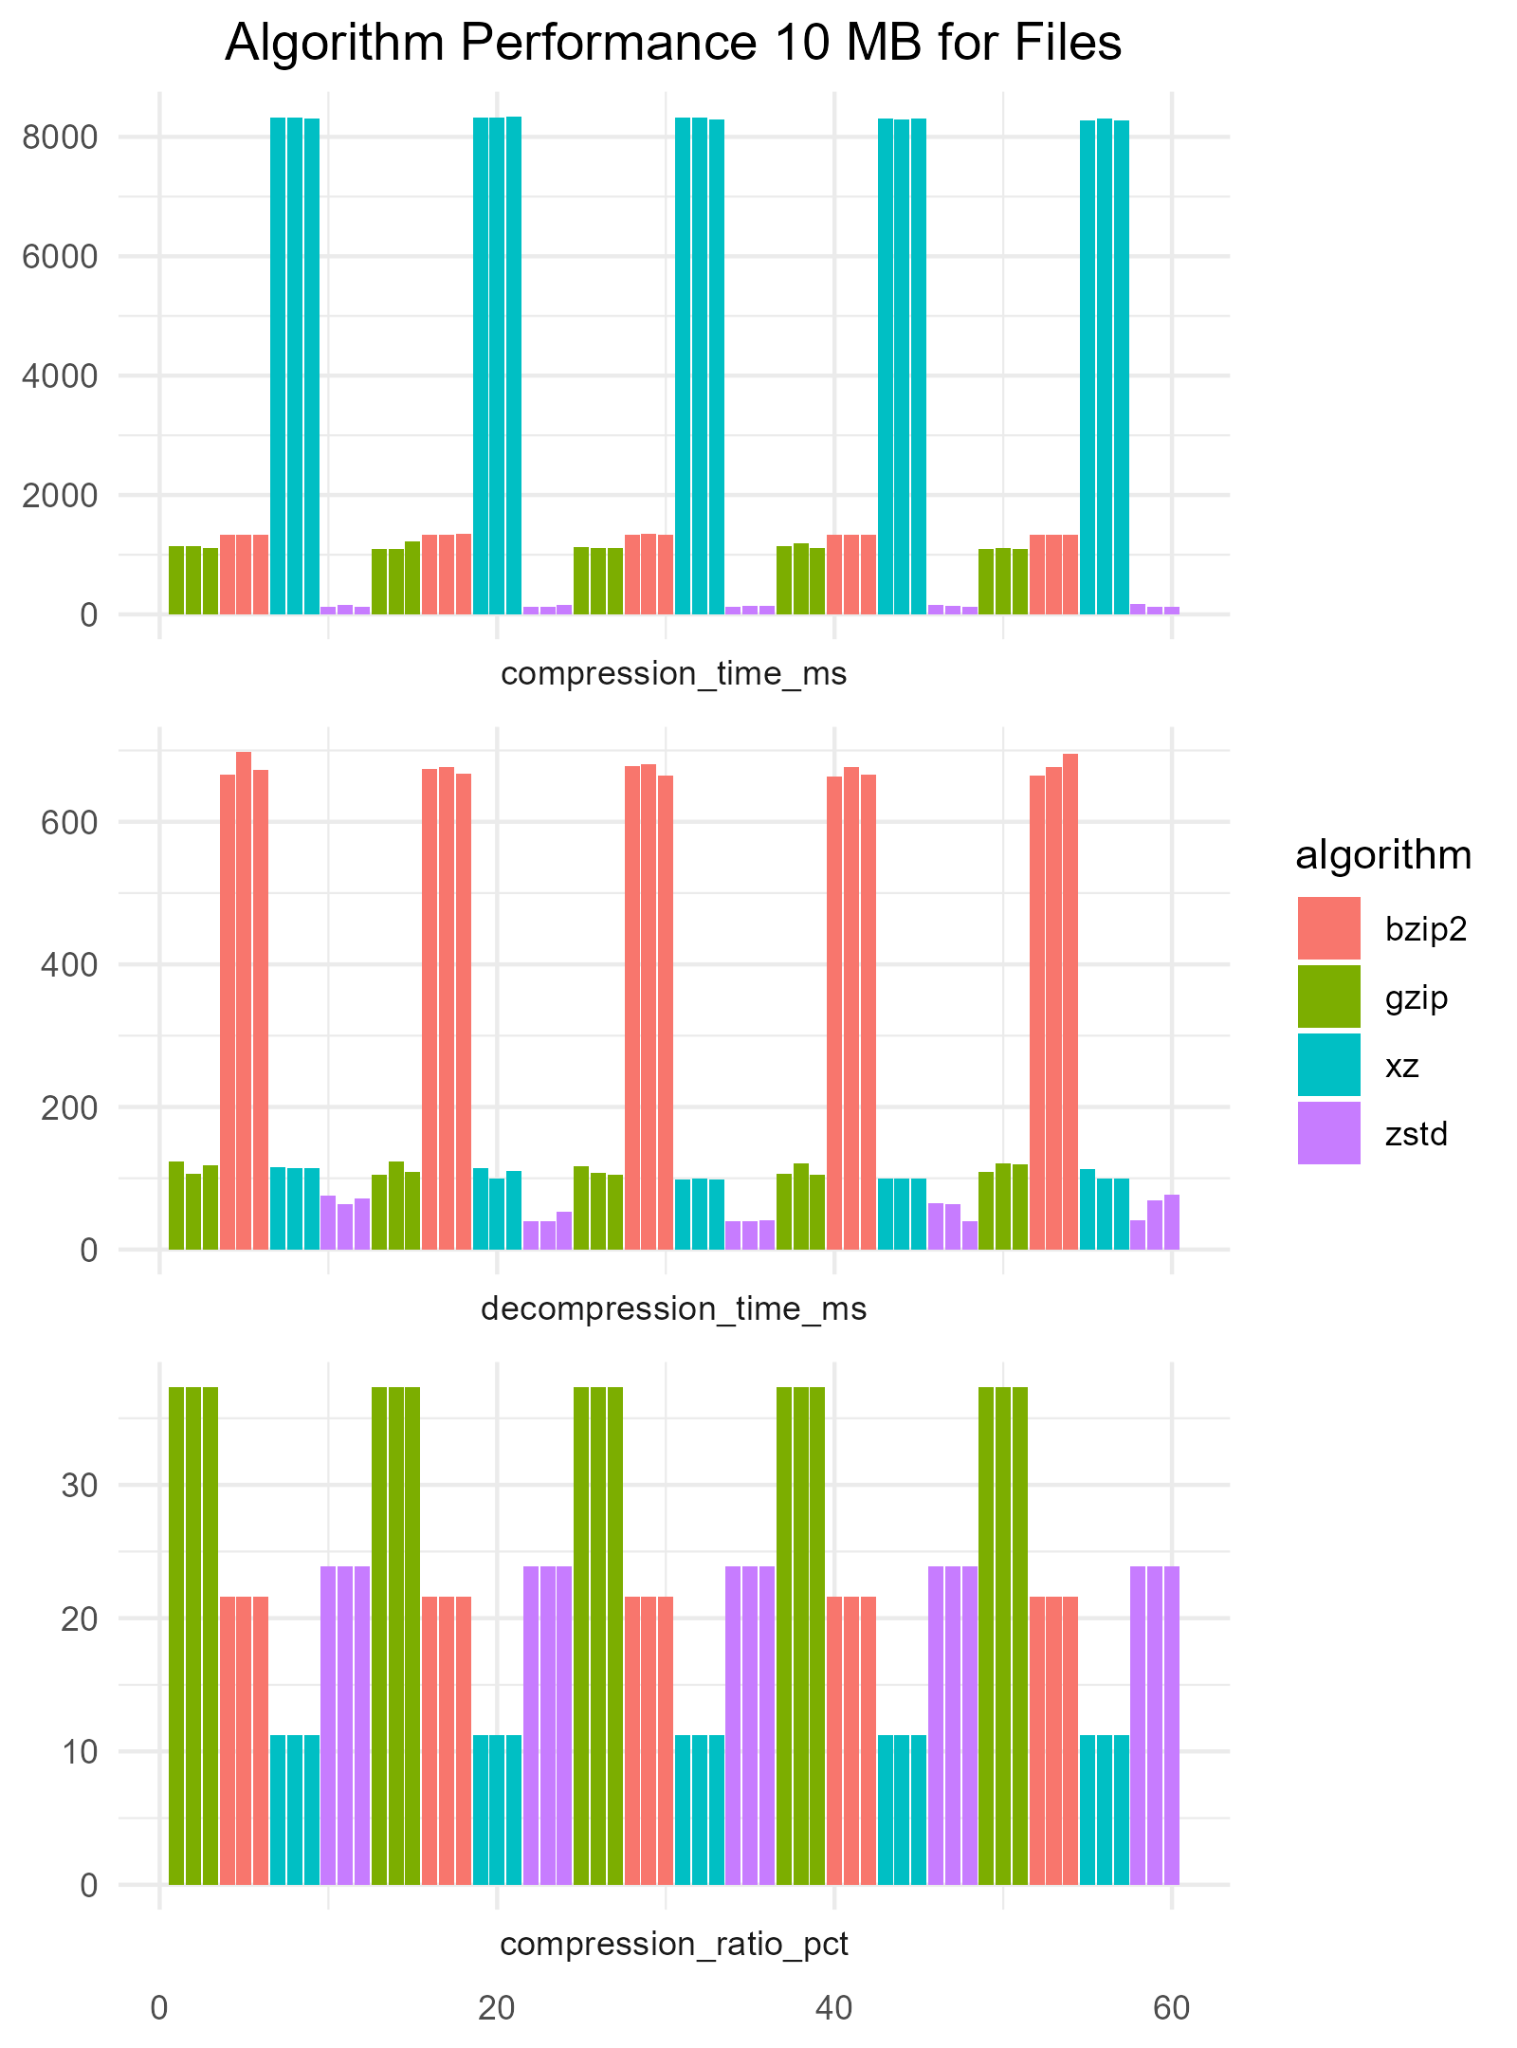
\includegraphics[width=\linewidth]{figures/image5}
  \caption{Desempenho dos algoritmos com arquivos de 10MB: tempo de compressão, descompressão e taxa de compressão.}
  \Description{Gráfico comparativo mostrando tempo de compressão, descompressão e taxa de compressão para arquivos de 10MB.}
  \label{fig:phase2_10mb}
\end{figure}

\begin{figure}[h]
  \centering
  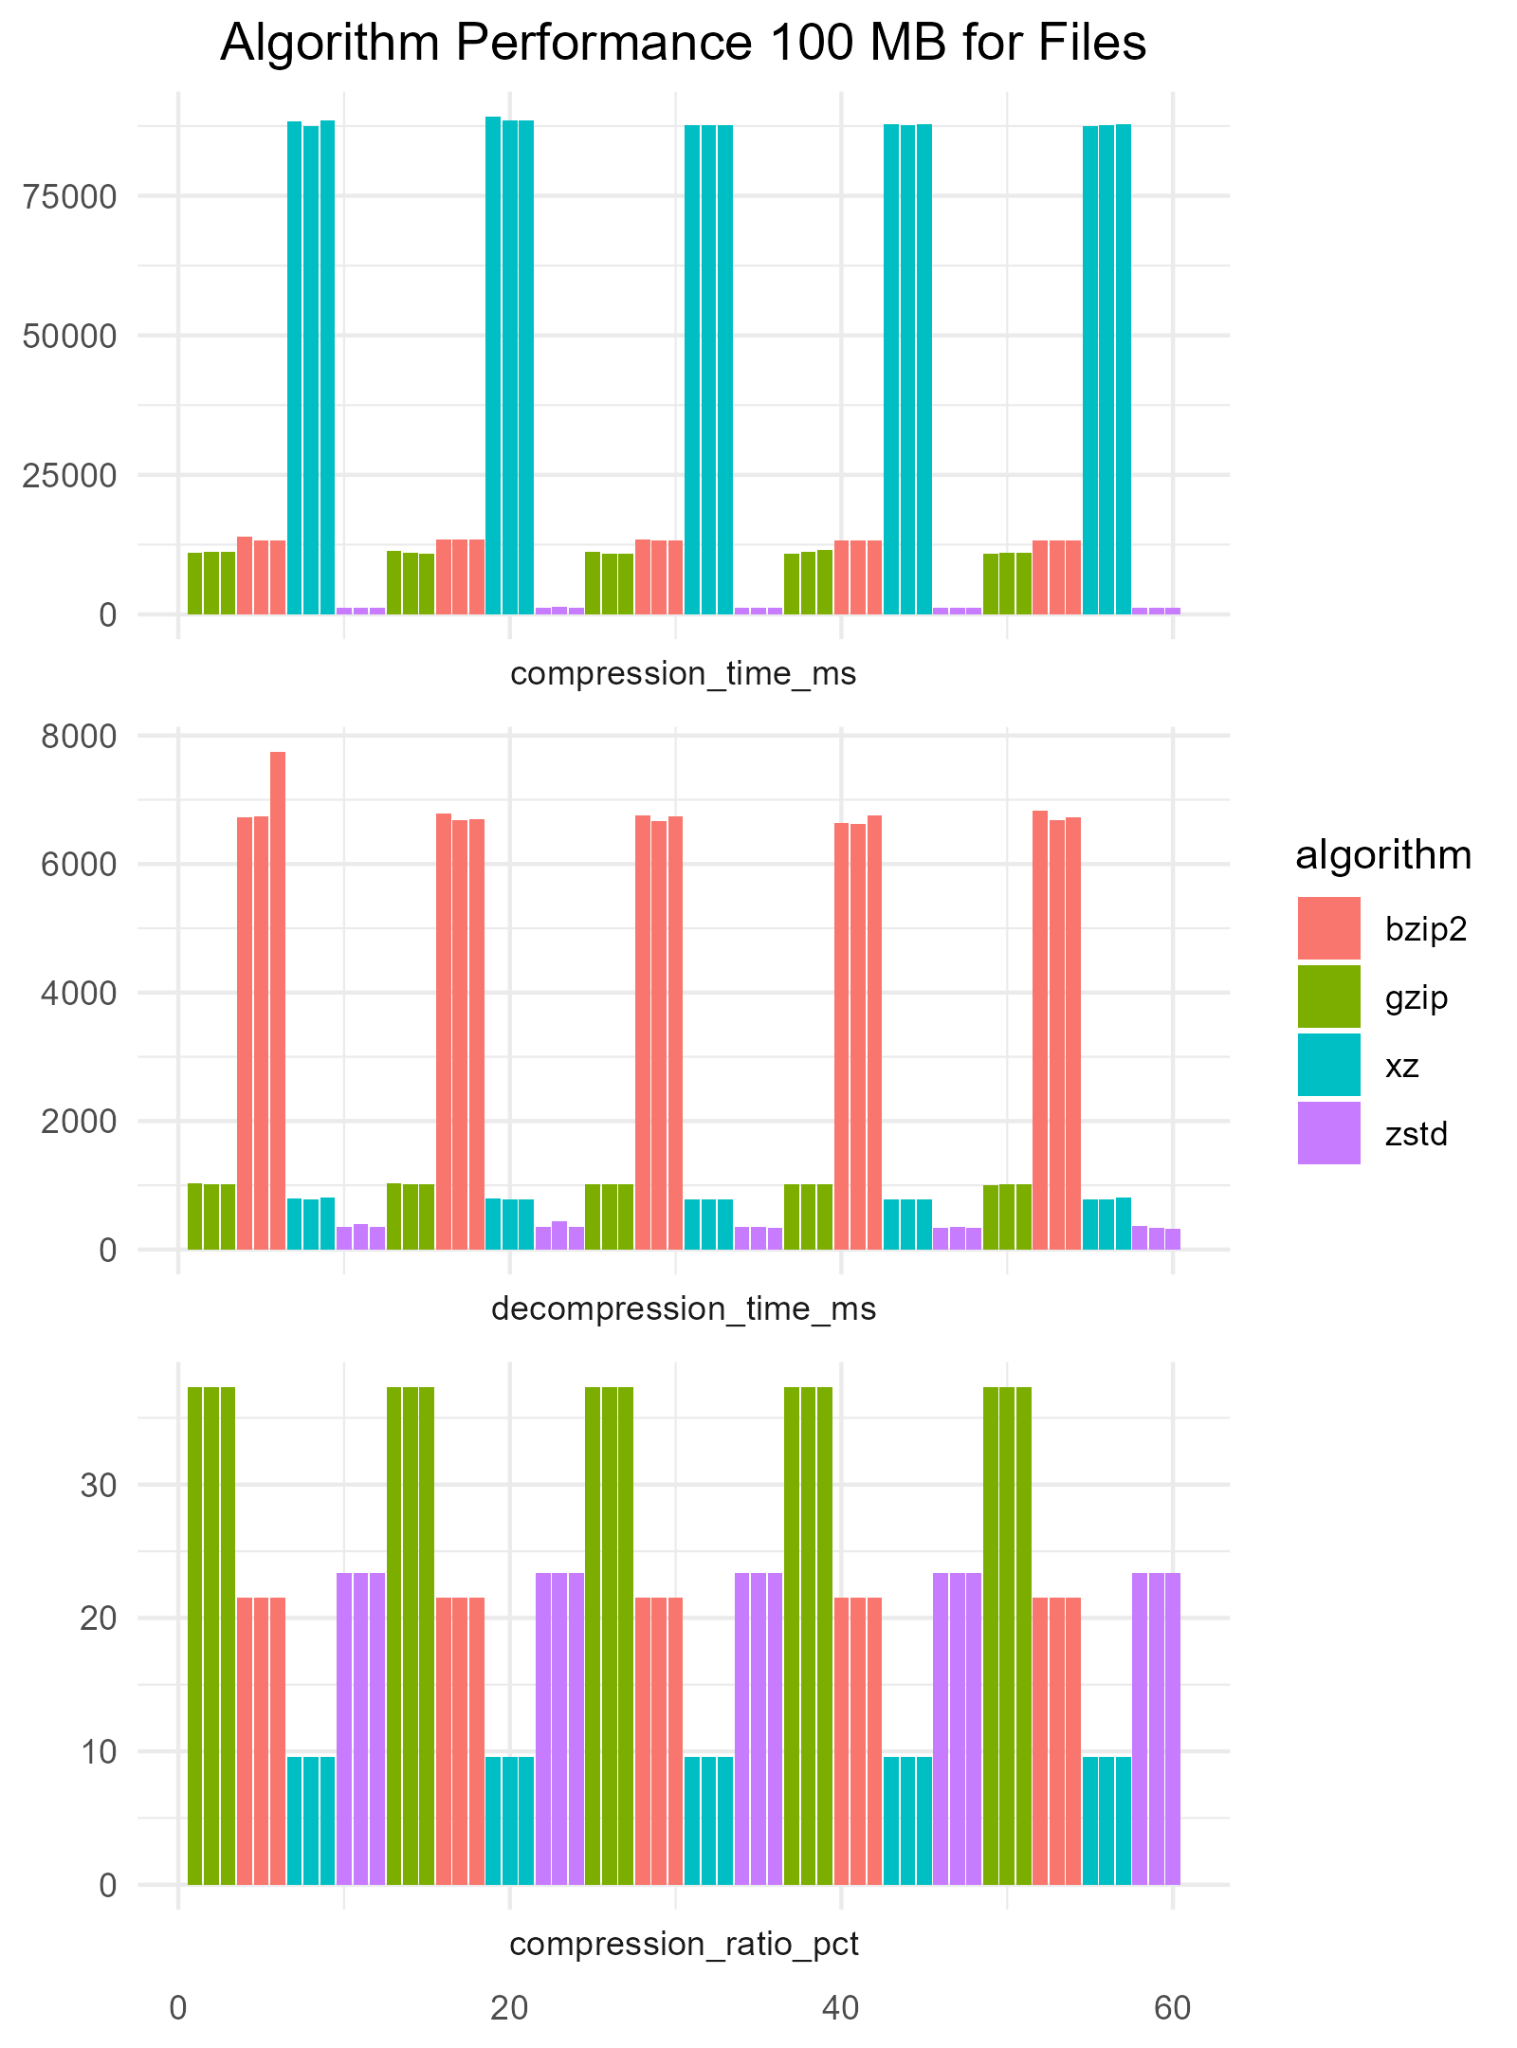
\includegraphics[width=\linewidth]{figures/image2}
  \caption{Desempenho dos algoritmos com arquivos de 100MB.}
  \Description{Gráfico comparativo para arquivos de 100MB.}
  \label{fig:phase2_100mb}
\end{figure}

\begin{figure}[h]
  \centering
  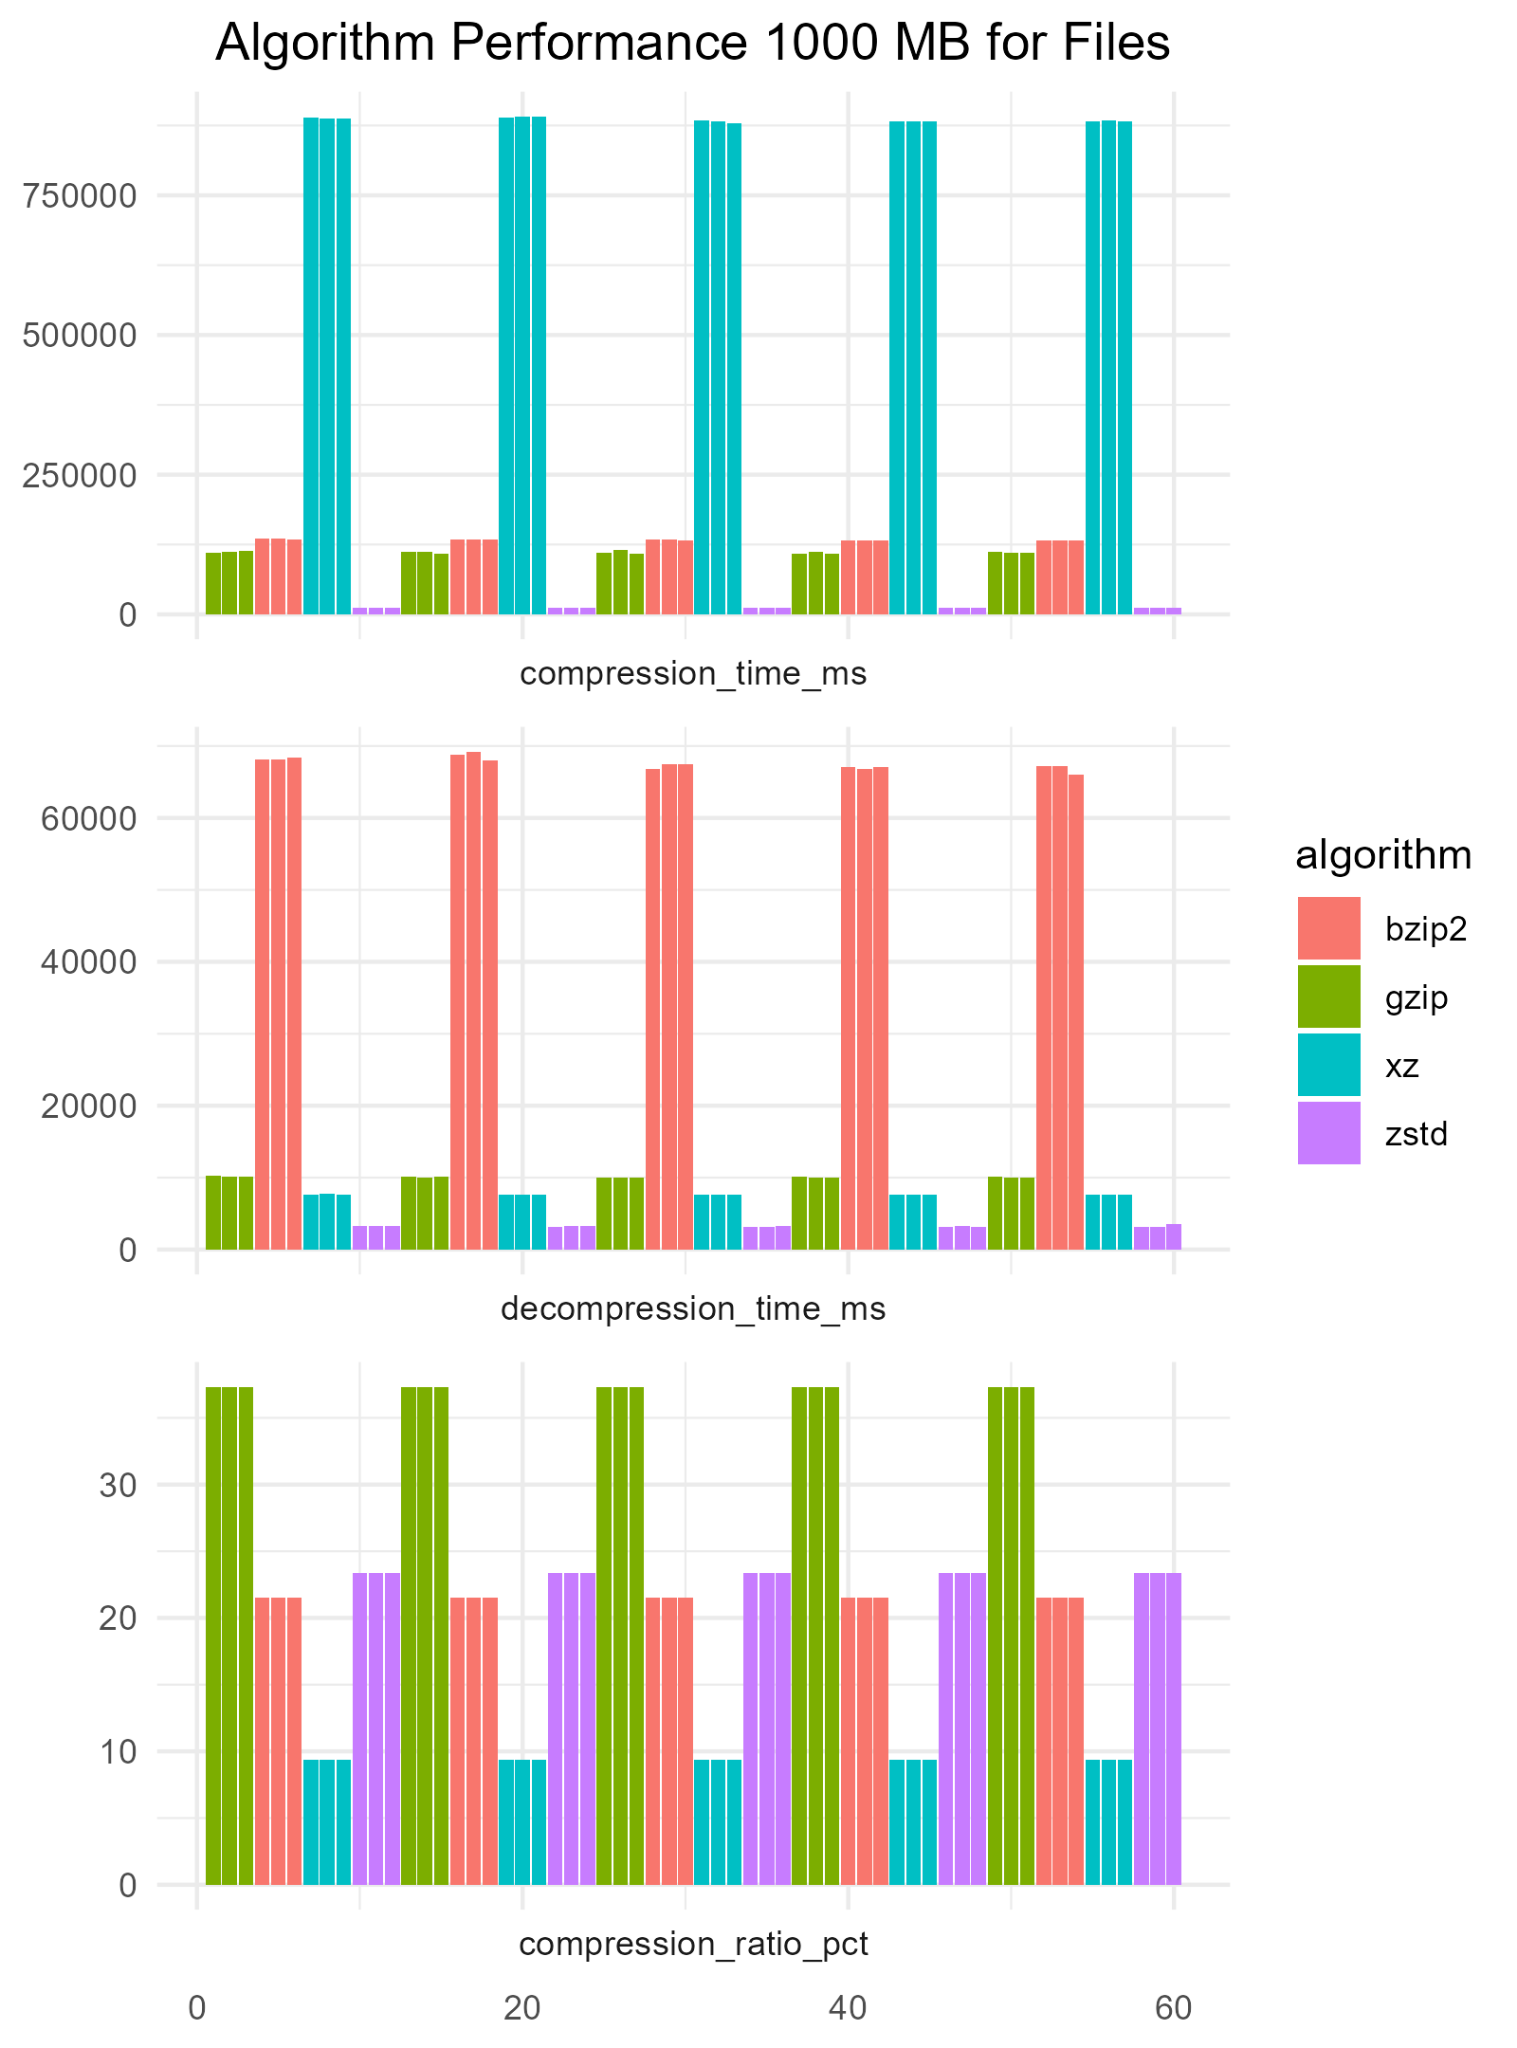
\includegraphics[width=\linewidth]{figures/image3}
  \caption{Desempenho dos algoritmos com arquivos de 1000MB.}
  \Description{Gráfico comparativo para arquivos de 1000MB.}
  \label{fig:phase2_1000mb}
\end{figure}

\textbf{Observações da Fase 2:}
\begin{itemize}
  \item O algoritmo XZ apresenta o maior tempo de compressão entre todos os algoritmos.
  \item O algoritmo BZIP2 apresenta o maior tempo de descompressão.
  \item Nesta etapa, a métrica de taxa de compressão estava invertida (quanto maior, pior). Isso foi corrigido na fase seguinte.
  \item Com quase 40\% de taxa, o GZIP possui o pior desempenho em eficiência de compressão, ou seja, 40\% do tamanho original não foi comprimido. O XZ apresentou apenas 10\% do tamanho original não comprimido.
\end{itemize}

\subsection{Resultados da Fase 3}

Na terceira fase, a metodologia foi refinada para garantir maior rigor científico. As principais mudanças foram:

\begin{itemize}
  \item \textbf{Arquivos pré-gerados:} Todos os arquivos de teste (de 1MB a 25MB) foram gerados uma única vez usando Cadeias de Markov e armazenados em \texttt{files.tar.xz}. Os mesmos arquivos são reutilizados em todas as execuções, eliminando a variabilidade da Fase 2.
  \item \textbf{Preload em cache:} Antes de cada bateria de testes, o arquivo é pré-carregado na memória com \texttt{cat arquivo > /dev/null}, eliminando o efeito de \textit{cold start} e garantindo que as medições reflitam apenas o tempo de processamento do algoritmo, sem interferência de I/O de disco.
  \item \textbf{Granularidade fina:} Em vez de apenas 3 tamanhos (10, 100, 1000MB), foram utilizados 25 tamanhos diferentes (1MB a 25MB), permitindo análise mais detalhada do comportamento dos algoritmos.
  \item \textbf{Métricas expandidas:} Além das métricas básicas, foram coletados dados de cache misses, page faults e chamadas de sistema de I/O.
\end{itemize}

Foram realizadas 3 execuções para cada combinação de algoritmo e tamanho de arquivo, totalizando 300 experimentos (4 algoritmos $\times$ 25 tamanhos $\times$ 3 repetições).

\subsubsection{Tempo de Compressão}

A Figura~\ref{fig:comp_time} apresenta o tempo de compressão em função do tamanho do arquivo. O algoritmo \textbf{xz} apresenta o maior tempo de compressão, crescendo linearmente de aproximadamente 0,6s para 1MB até 21,5s para 25MB. Em contraste, o \textbf{zstd} mantém tempos extremamente baixos (0,01s a 0,26s), sendo até 80 vezes mais rápido que o xz para arquivos grandes.

\begin{figure}[h]
  \centering
  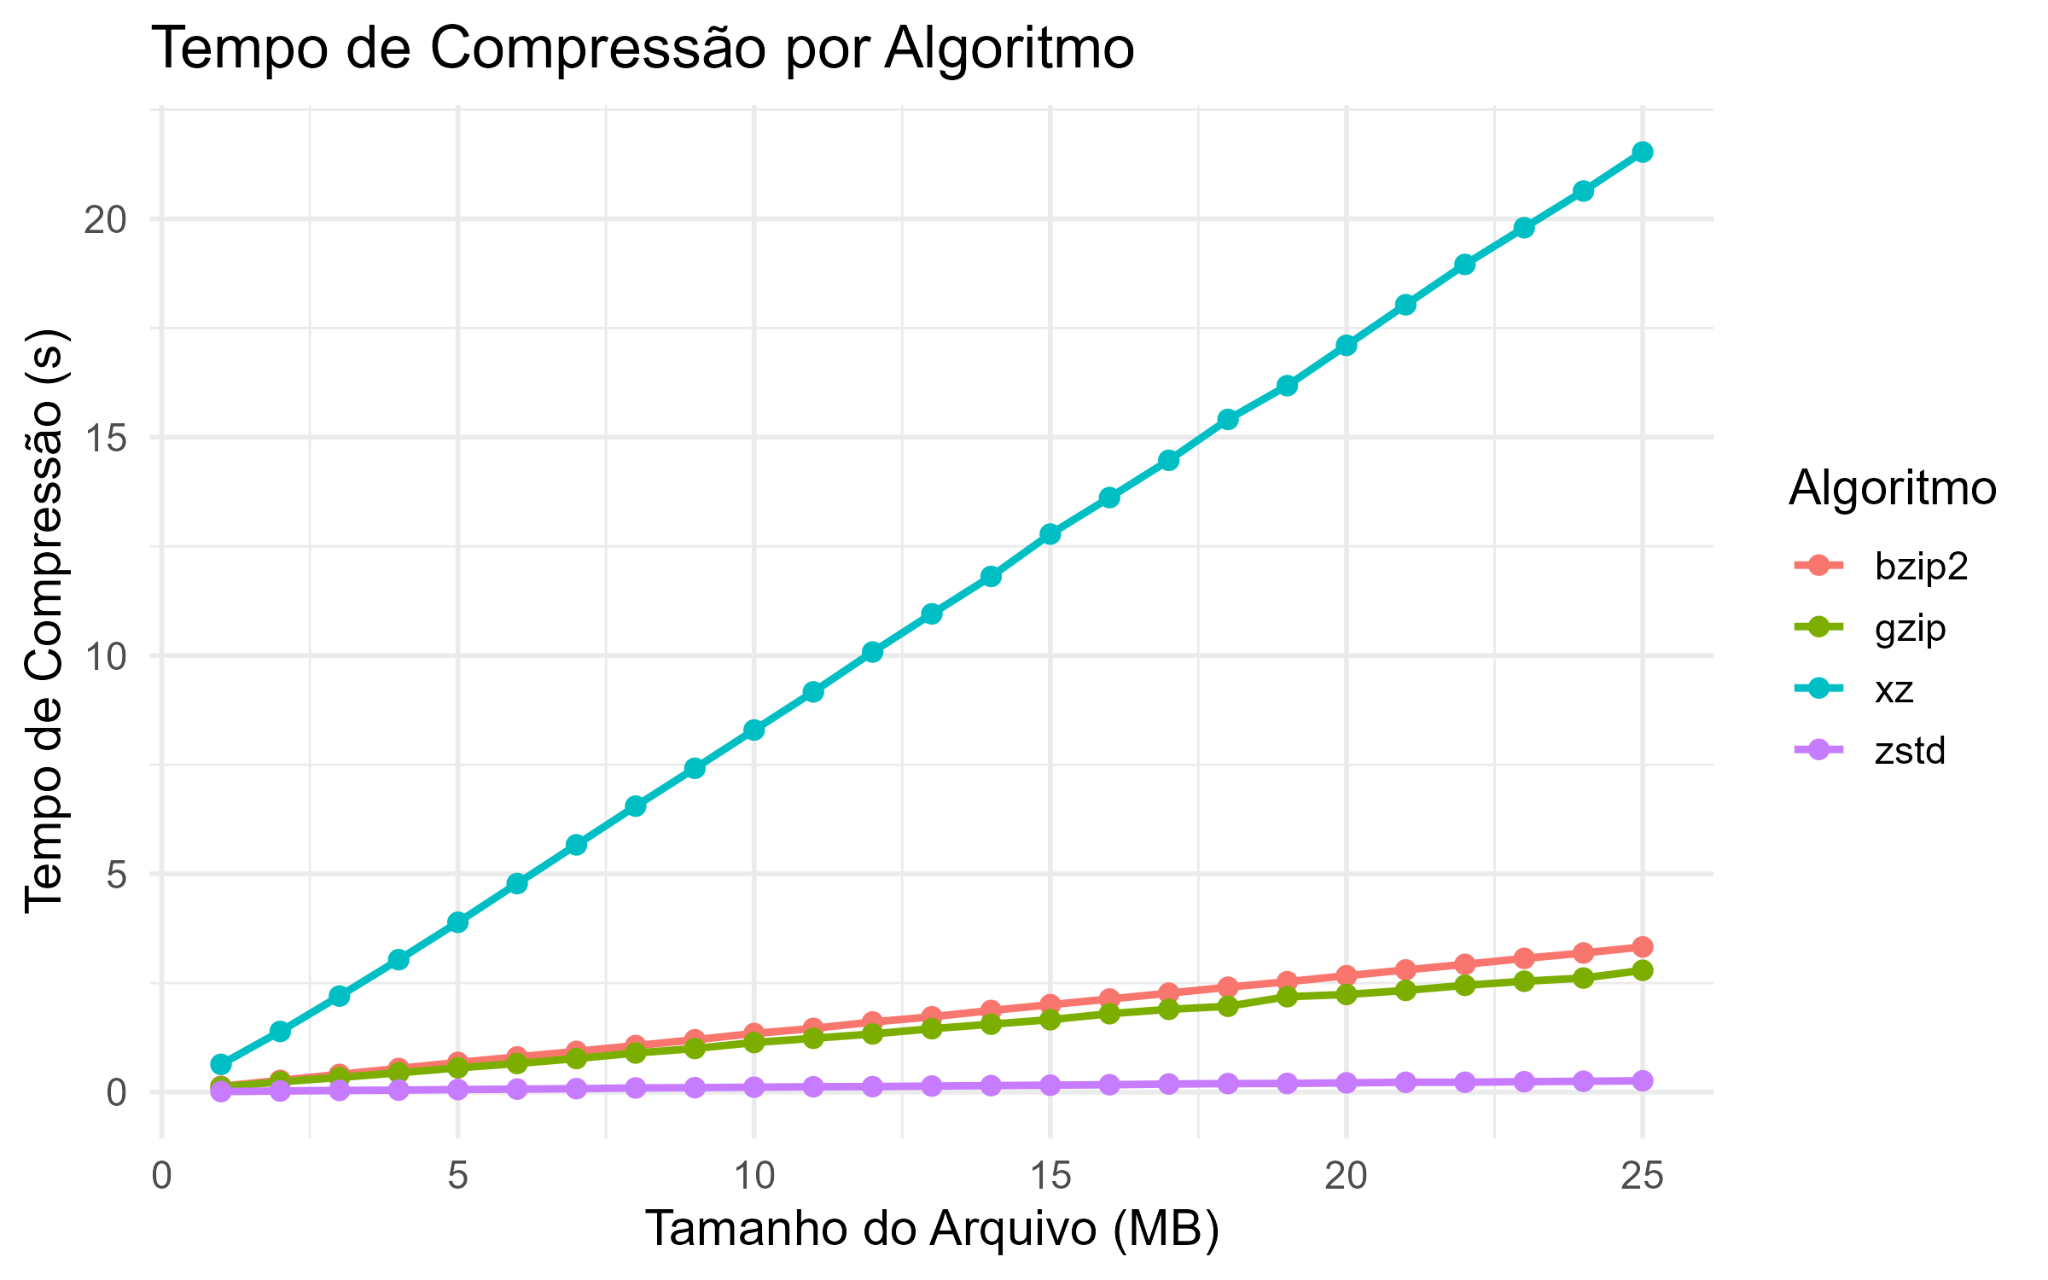
\includegraphics[width=\linewidth]{figures/image9}
  \caption{Tempo de compressão por algoritmo em função do tamanho do arquivo.}
  \Description{Gráfico mostrando tempo de compressão para cada algoritmo, com xz apresentando os maiores tempos e zstd os menores.}
  \label{fig:comp_time}
\end{figure}

A Figura~\ref{fig:reg_comp_time} apresenta os mesmos dados com regressão linear e projeção para arquivos de até 35MB, permitindo estimar o comportamento para arquivos maiores.

\begin{figure}[h]
  \centering
  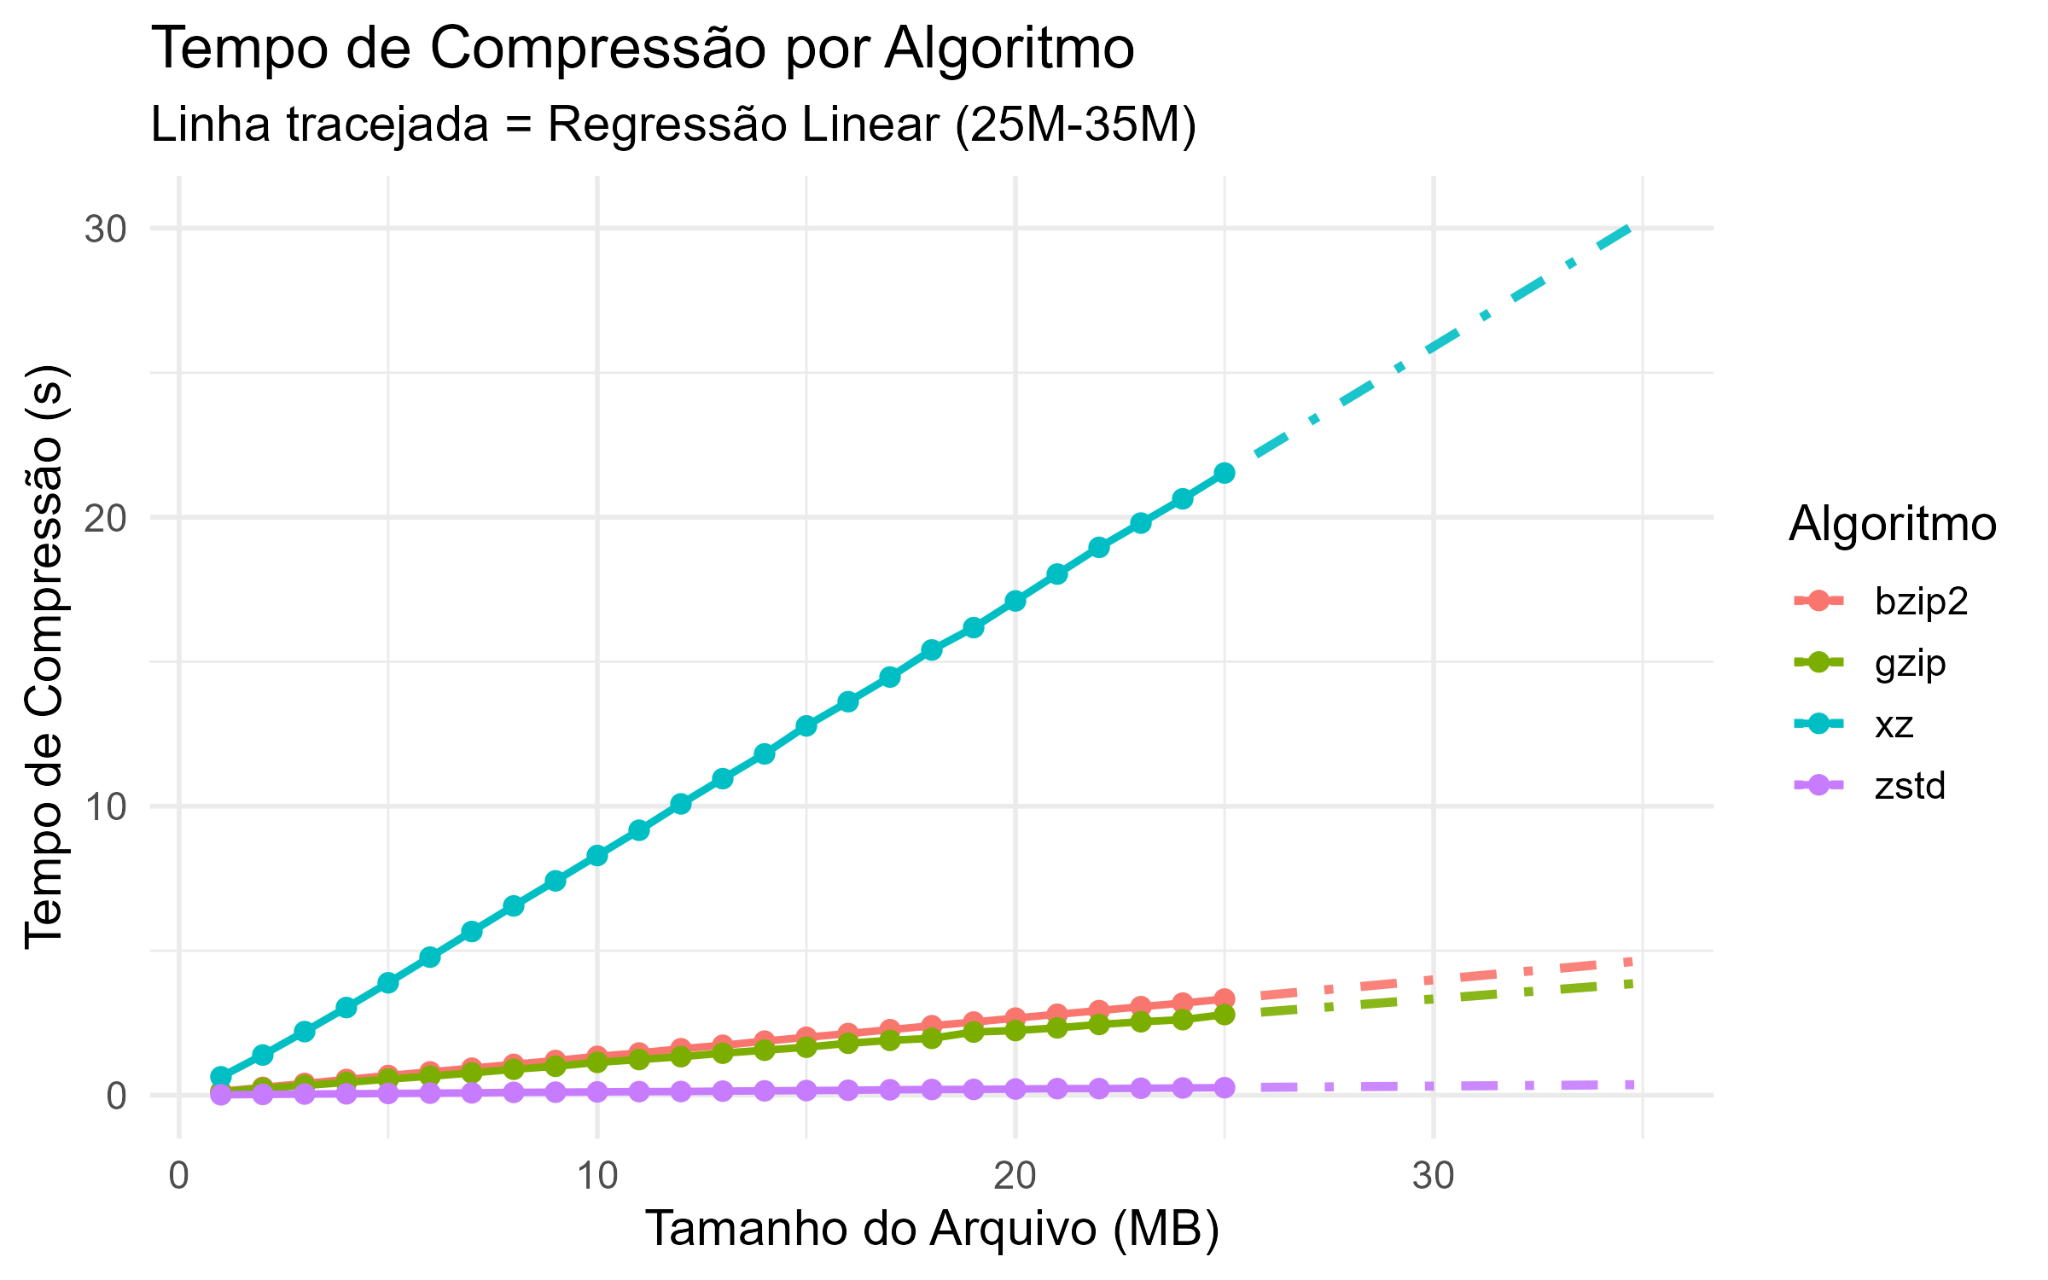
\includegraphics[width=\linewidth]{figures/image1}
  \caption{Tempo de compressão com regressão linear (projeção 25M-35M).}
  \Description{Gráfico de regressão linear do tempo de compressão com projeção para arquivos maiores.}
  \label{fig:reg_comp_time}
\end{figure}

\subsubsection{Tempo de Descompressão}

A Figura~\ref{fig:decomp_time} mostra o tempo de descompressão. Diferentemente da compressão, o \textbf{bzip2} apresenta os piores tempos de descompressão, chegando a 1,7s para arquivos de 25MB. Os demais algoritmos (gzip, xz e zstd) mantêm tempos de descompressão similares e baixos, com o zstd novamente liderando com tempos inferiores a 0,1s.

\begin{figure}[h]
  \centering
  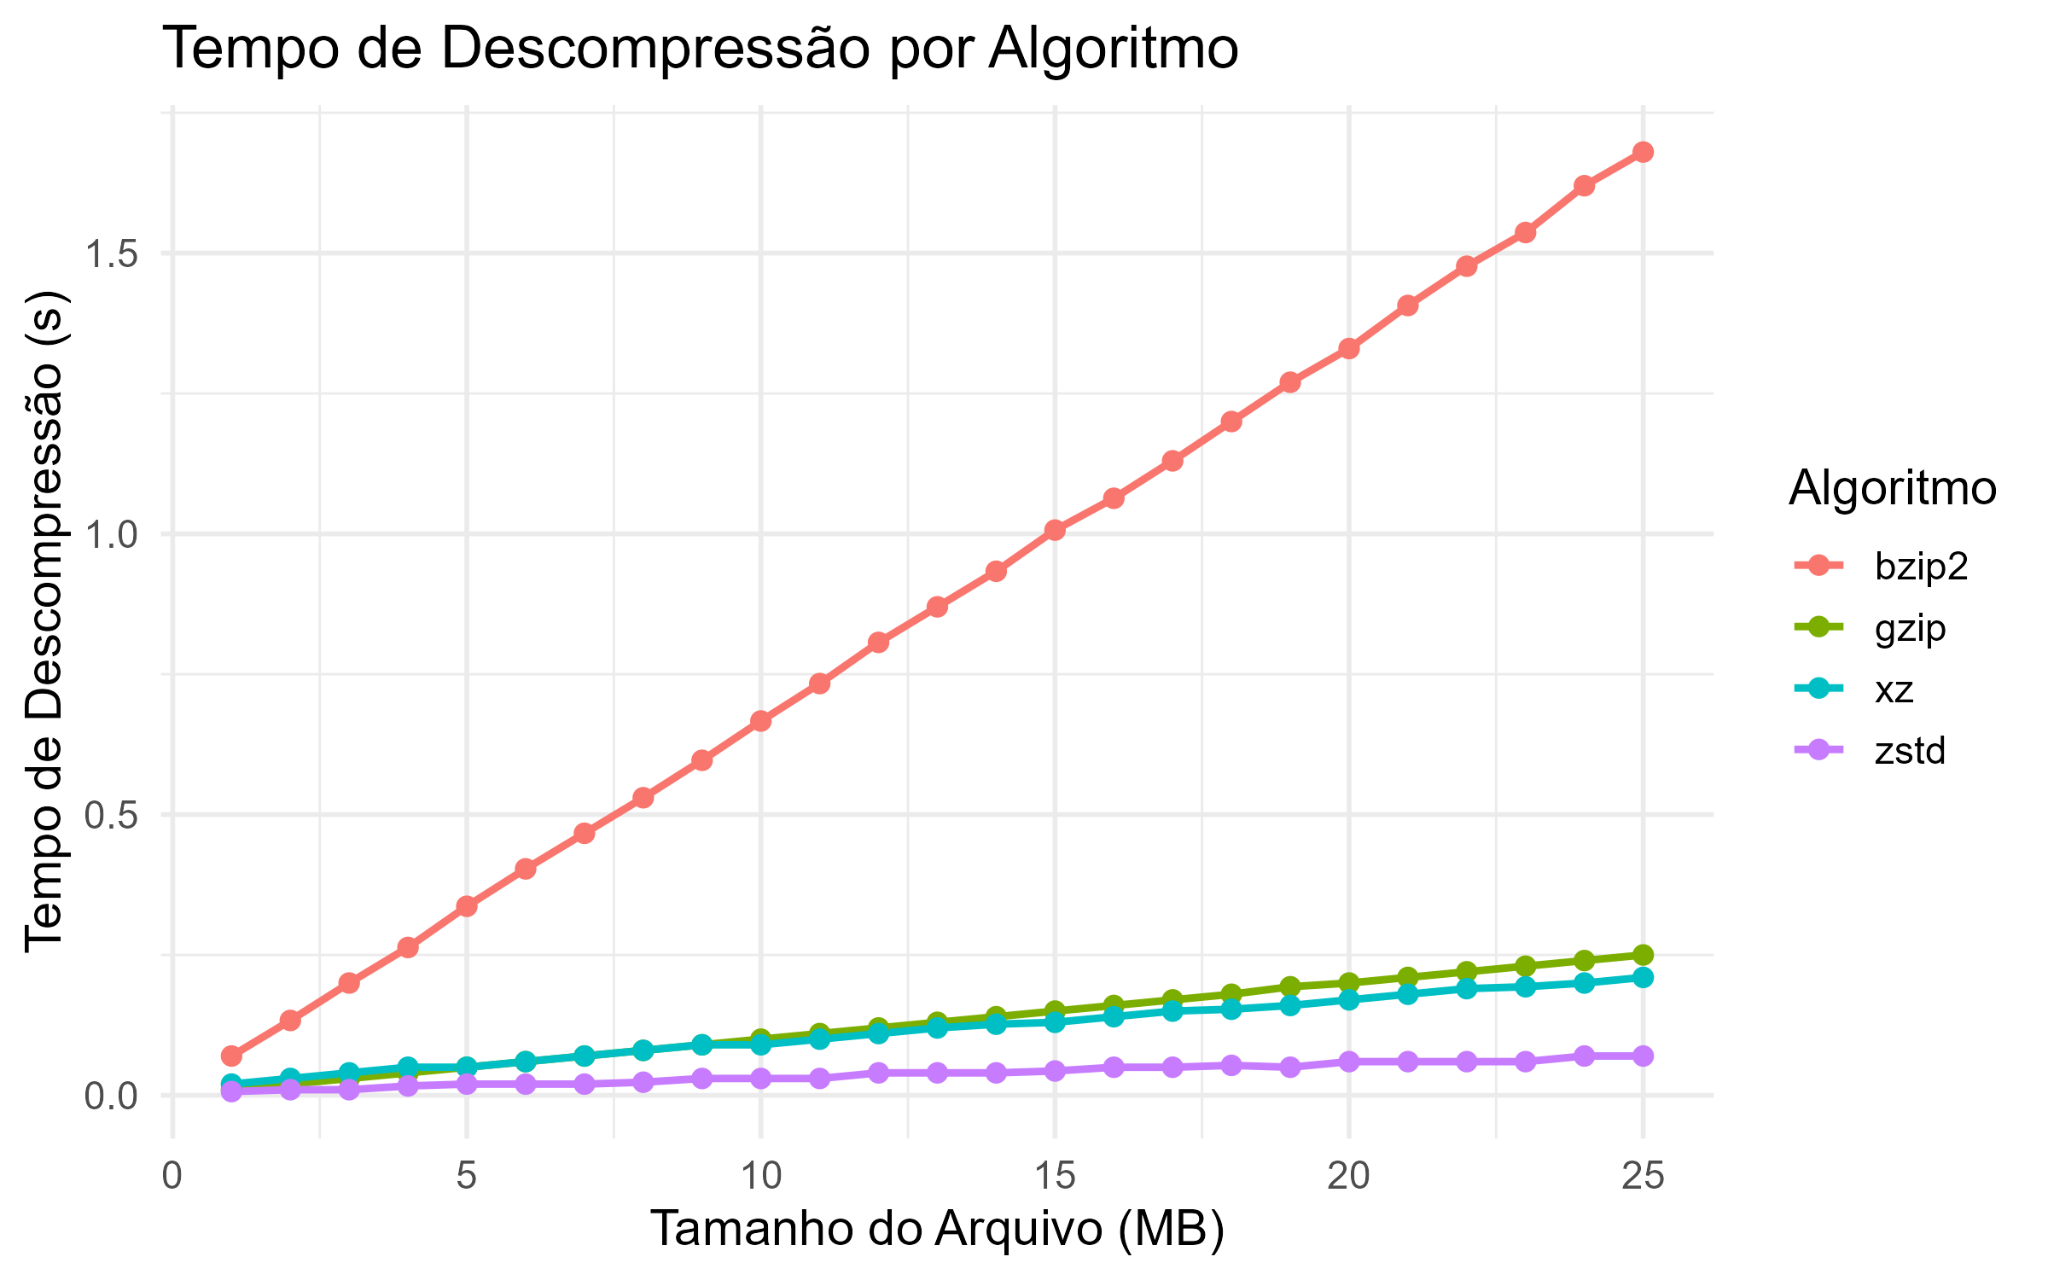
\includegraphics[width=\linewidth]{figures/image11}
  \caption{Tempo de descompressão por algoritmo em função do tamanho do arquivo.}
  \Description{Gráfico mostrando tempo de descompressão, com bzip2 apresentando os maiores tempos.}
  \label{fig:decomp_time}
\end{figure}

A Figura~\ref{fig:reg_decomp_time} apresenta os mesmos dados com regressão linear e projeção para arquivos maiores.

\begin{figure}[h]
  \centering
  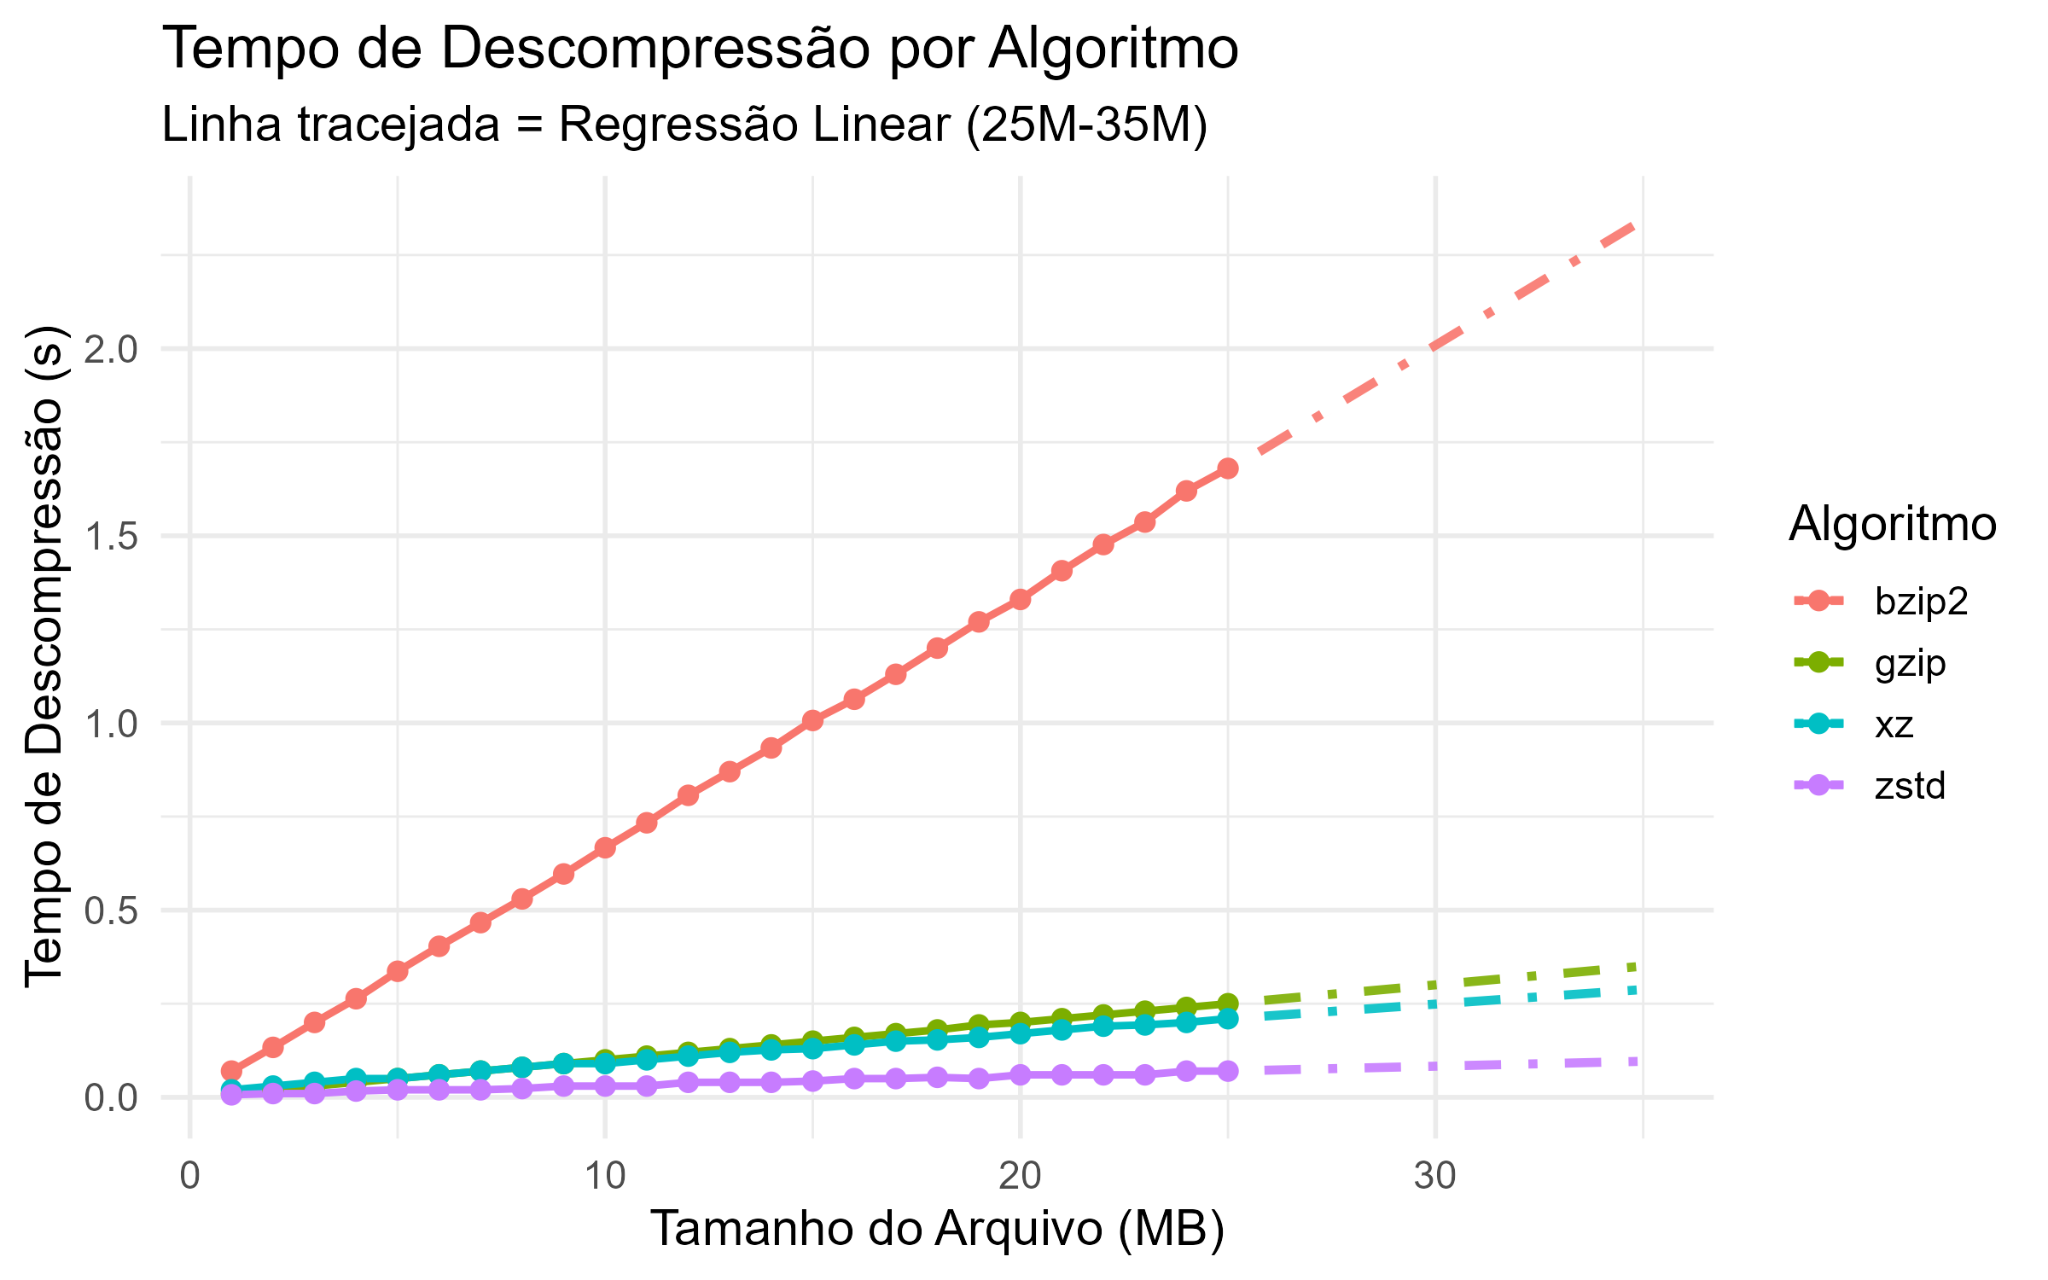
\includegraphics[width=\linewidth]{figures/image7}
  \caption{Tempo de descompressão com regressão linear (projeção 25M-35M).}
  \Description{Gráfico de regressão linear do tempo de descompressão com projeção.}
  \label{fig:reg_decomp_time}
\end{figure}

\subsubsection{Taxa de Compressão}

A Figura~\ref{fig:comp_rate} apresenta a taxa de compressão (quanto maior, melhor). O \textbf{xz} atinge as melhores taxas, comprimindo até 90\% do arquivo original para tamanhos maiores. O \textbf{gzip} apresenta desempenho consistentemente inferior, mantendo-se em torno de 63\% de compressão independentemente do tamanho do arquivo.

\begin{figure}[h]
  \centering
  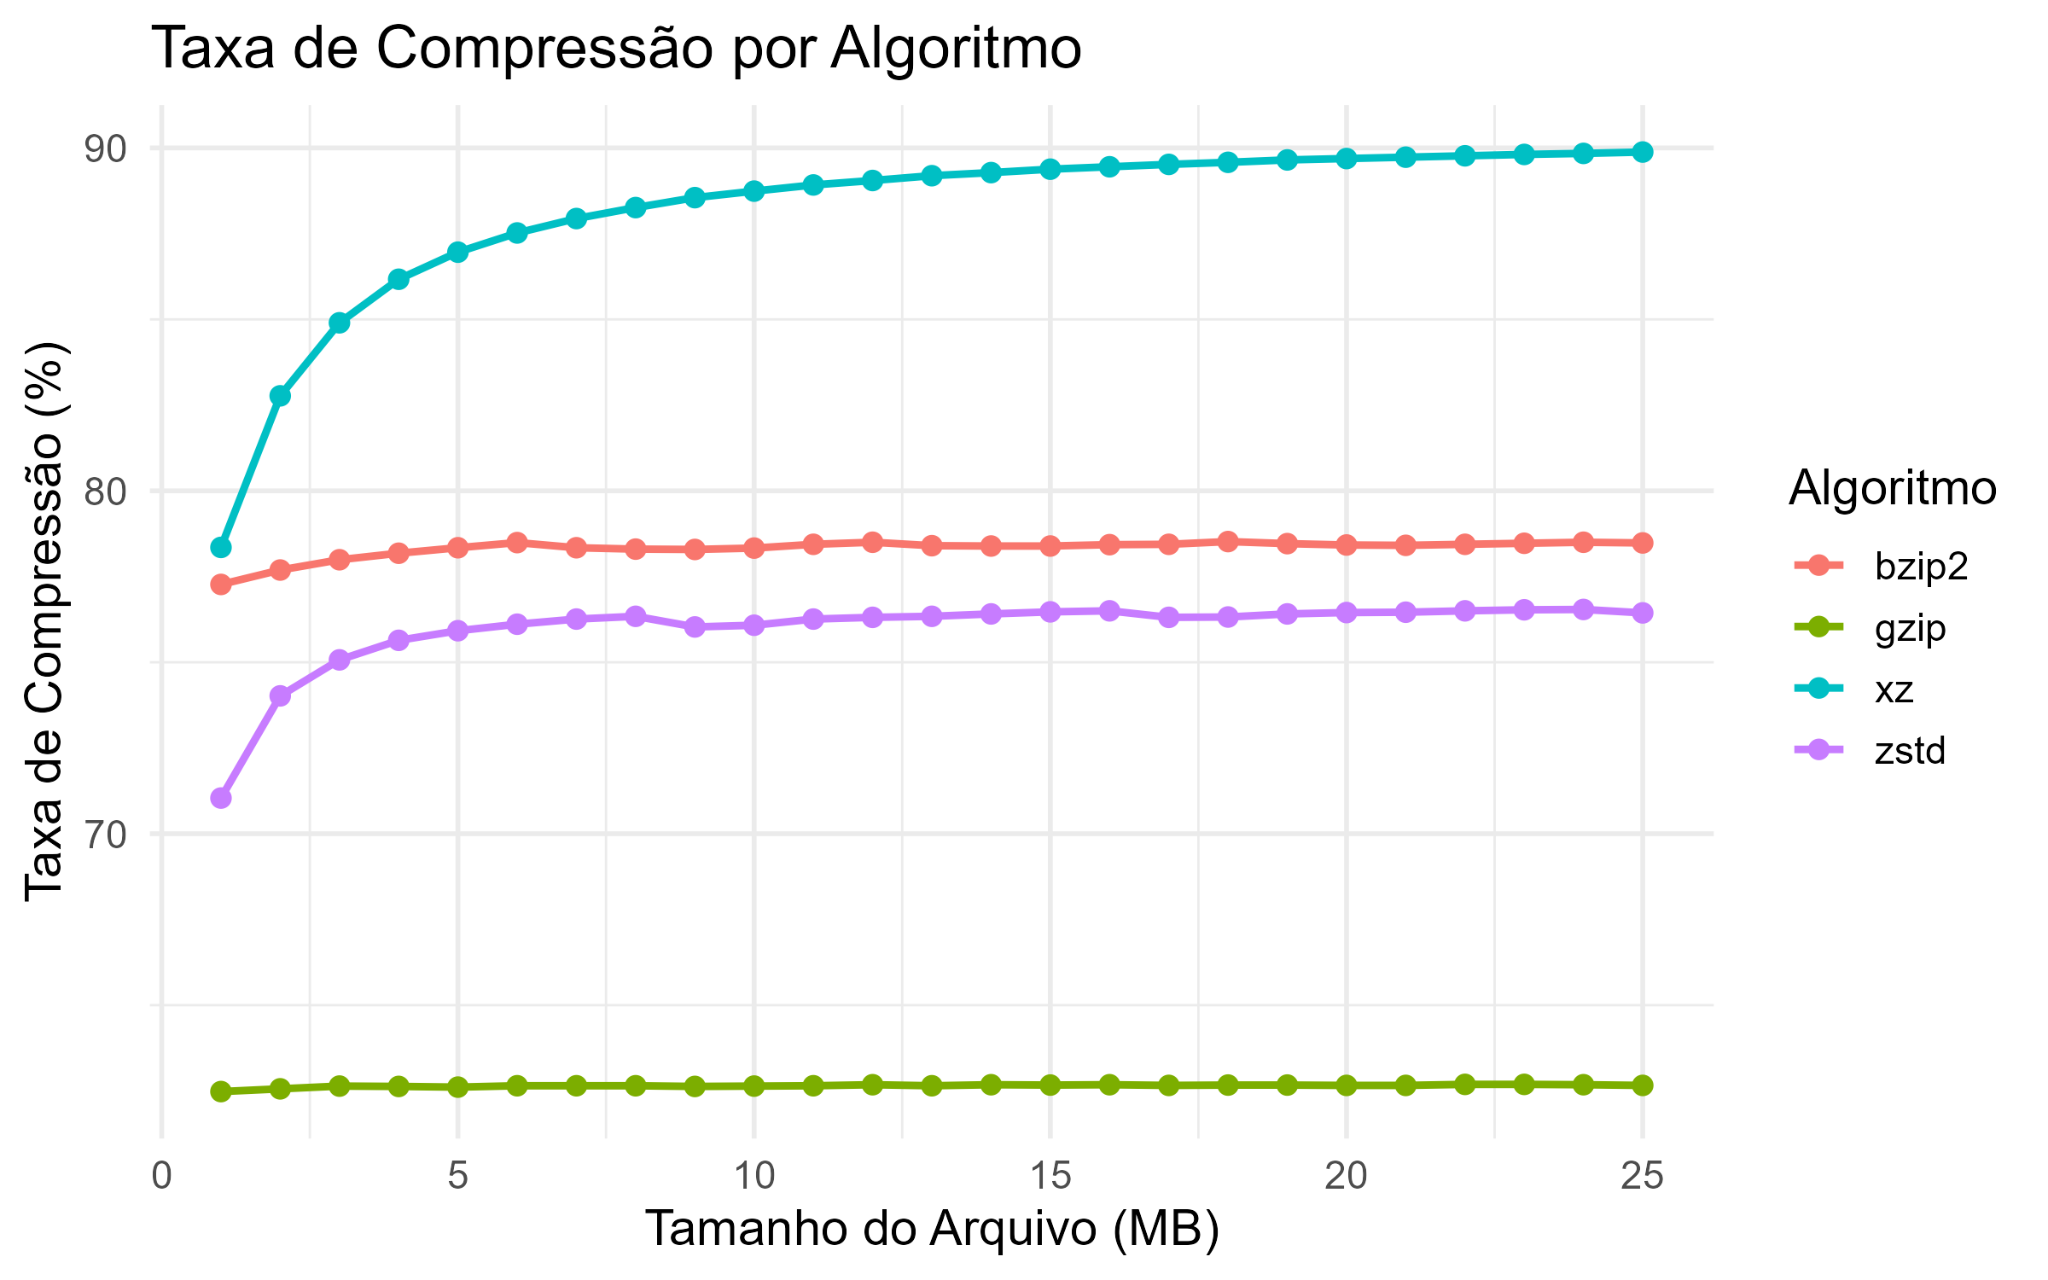
\includegraphics[width=\linewidth]{figures/image6}
  \caption{Taxa de compressão por algoritmo em função do tamanho do arquivo.}
  \Description{Gráfico mostrando taxa de compressão, com xz atingindo as melhores taxas e gzip as piores.}
  \label{fig:comp_rate}
\end{figure}

A Figura~\ref{fig:reg_rate} apresenta a taxa de compressão com regressão SPLINE e projeção para arquivos maiores.

\begin{figure}[h]
  \centering
  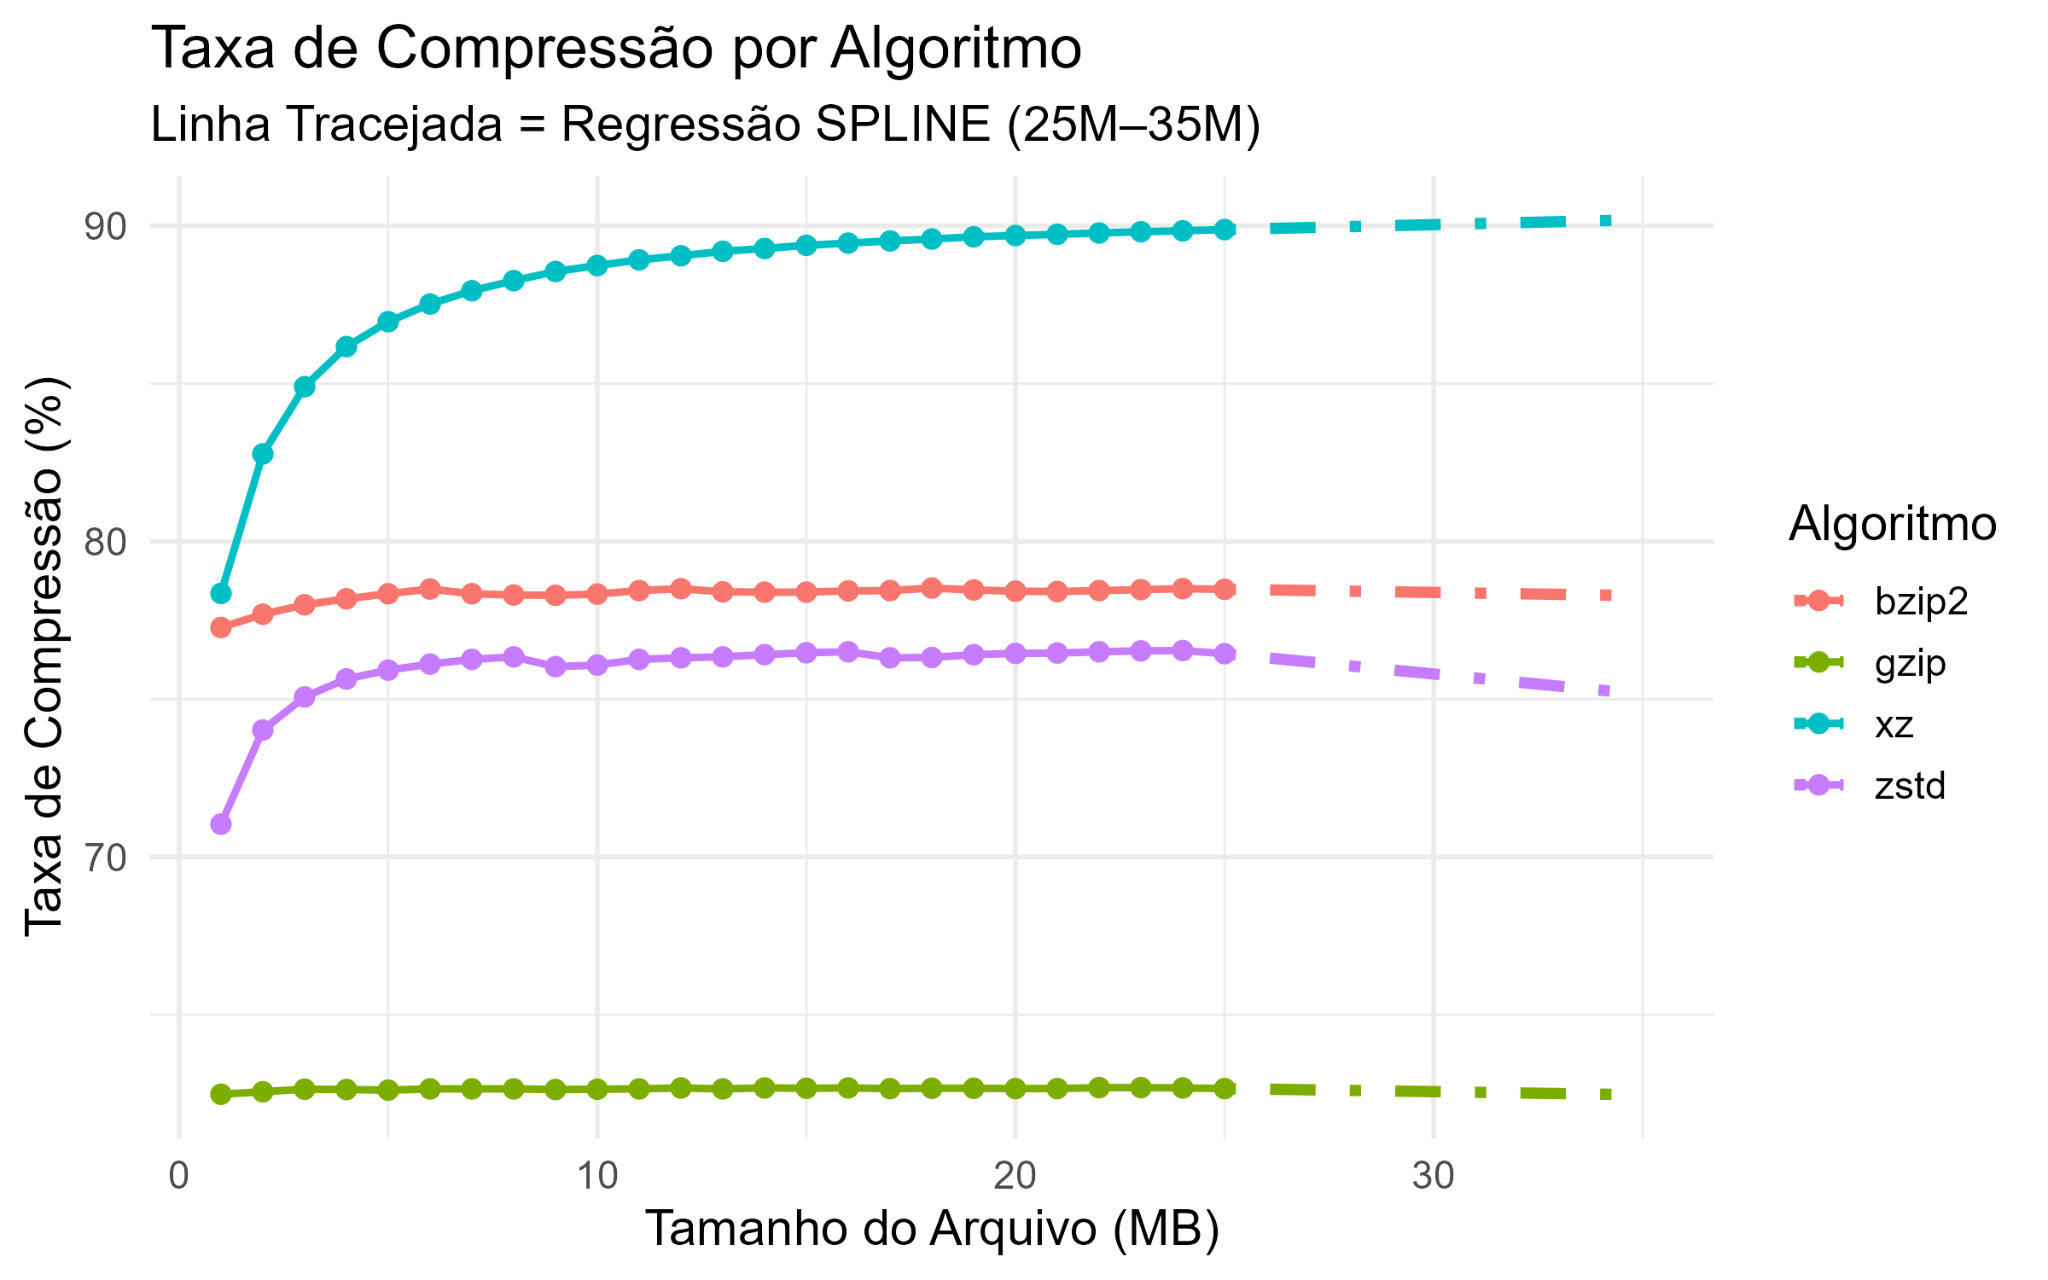
\includegraphics[width=\linewidth]{figures/image4}
  \caption{Taxa de compressão com regressão SPLINE (projeção 25M-35M).}
  \Description{Gráfico de regressão da taxa de compressão com projeção.}
  \label{fig:reg_rate}
\end{figure}

\subsubsection{Análise com Intervalo de Confiança}

As Figuras~\ref{fig:ic_comp} e~\ref{fig:ic_comp2} apresentam os tempos de compressão com intervalo de confiança de 95\%, demonstrando a estabilidade das medições. As barras de erro são praticamente invisíveis, indicando alta reprodutibilidade dos experimentos.

\begin{figure}[h]
  \centering
  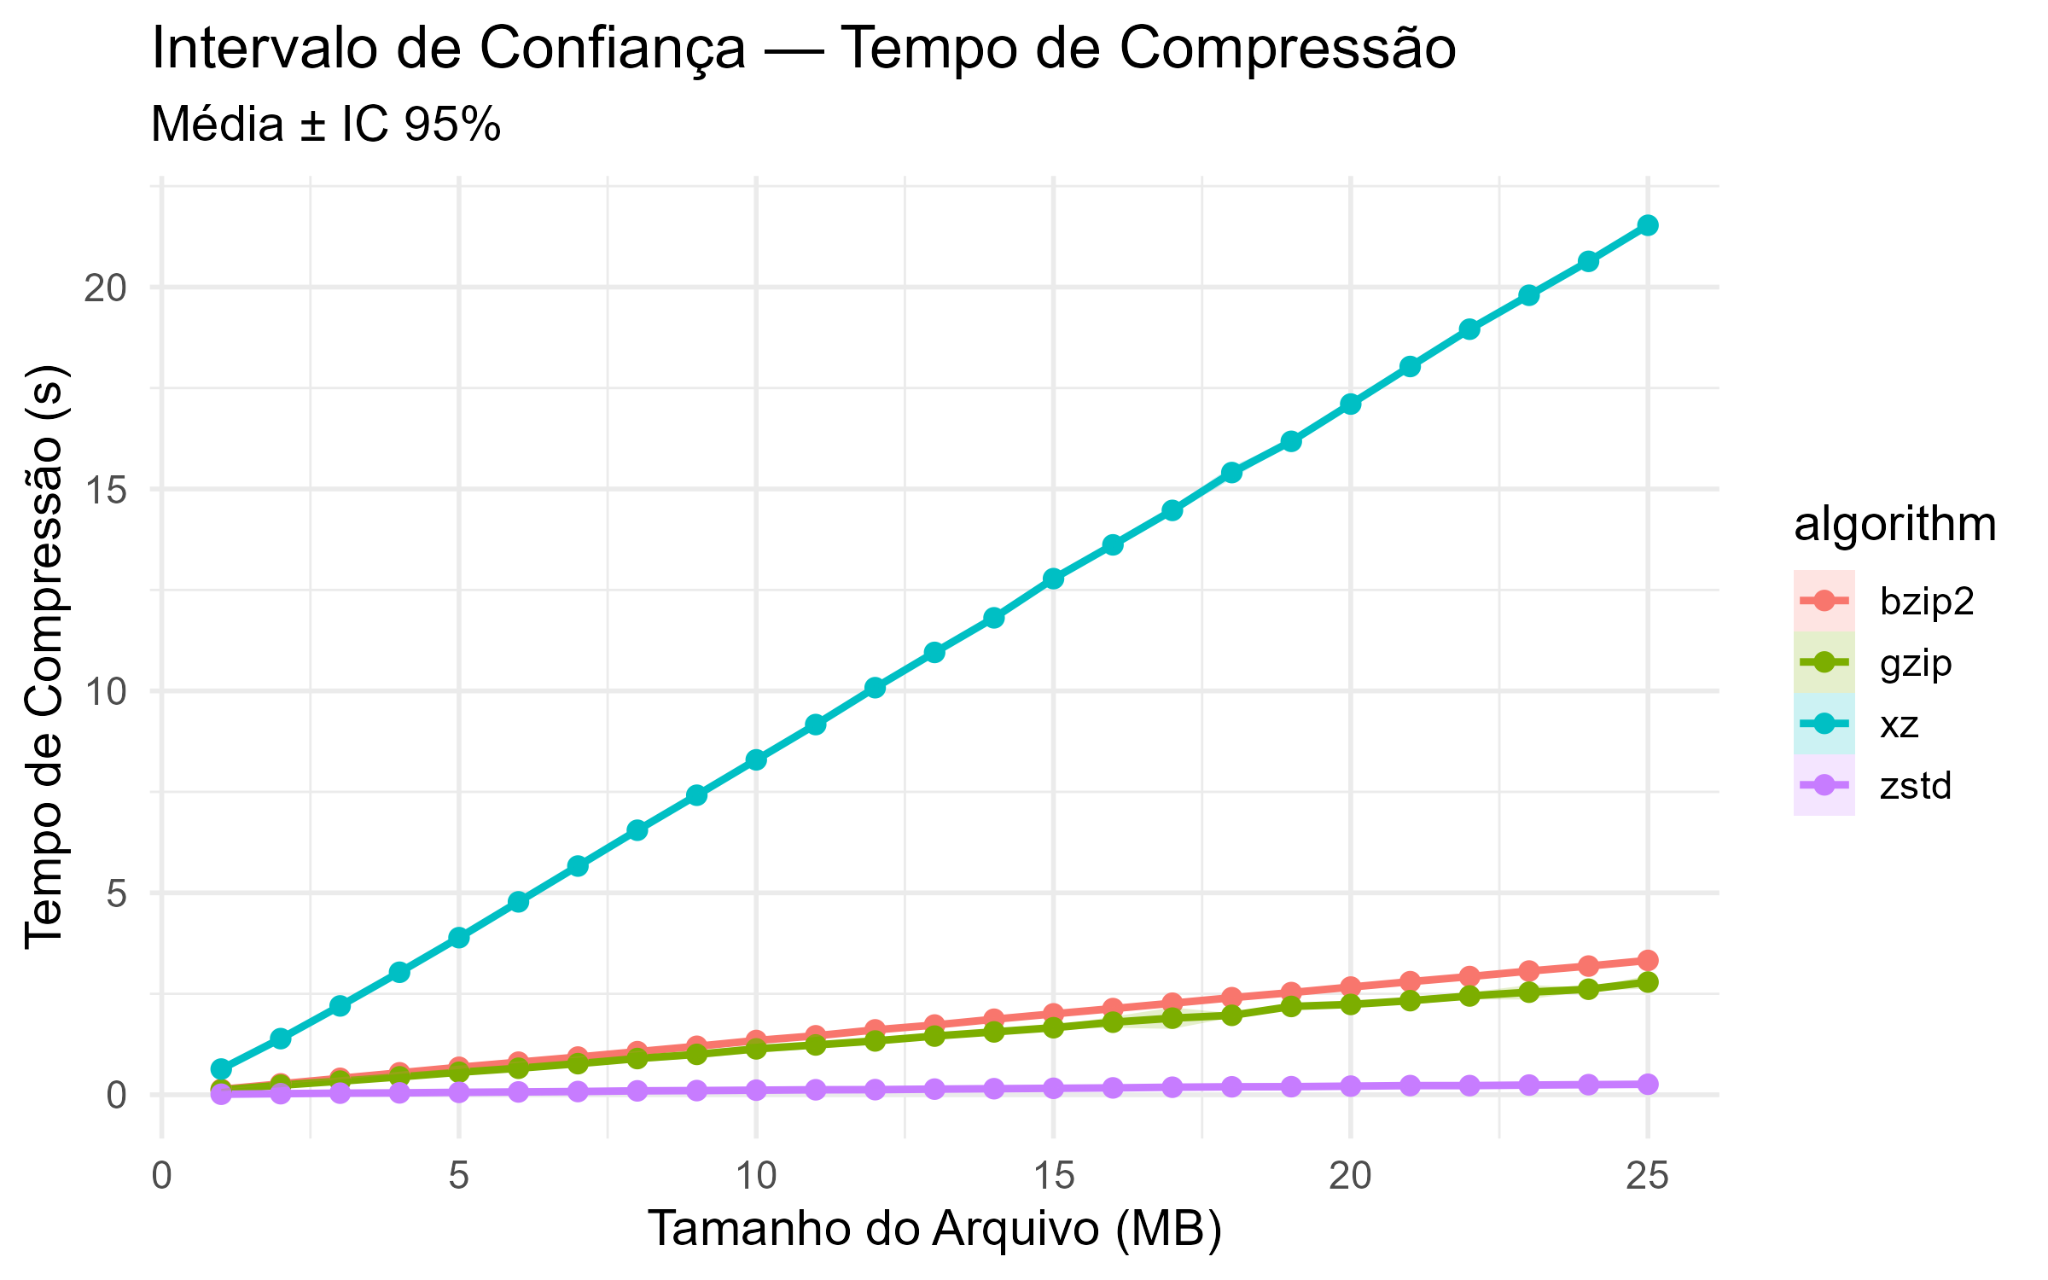
\includegraphics[width=\linewidth]{figures/image8}
  \caption{Intervalo de confiança (95\%) para tempo de compressão.}
  \Description{Gráfico com barras de erro mostrando a estabilidade das medições de tempo de compressão.}
  \label{fig:ic_comp}
\end{figure}

\begin{figure}[h]
  \centering
  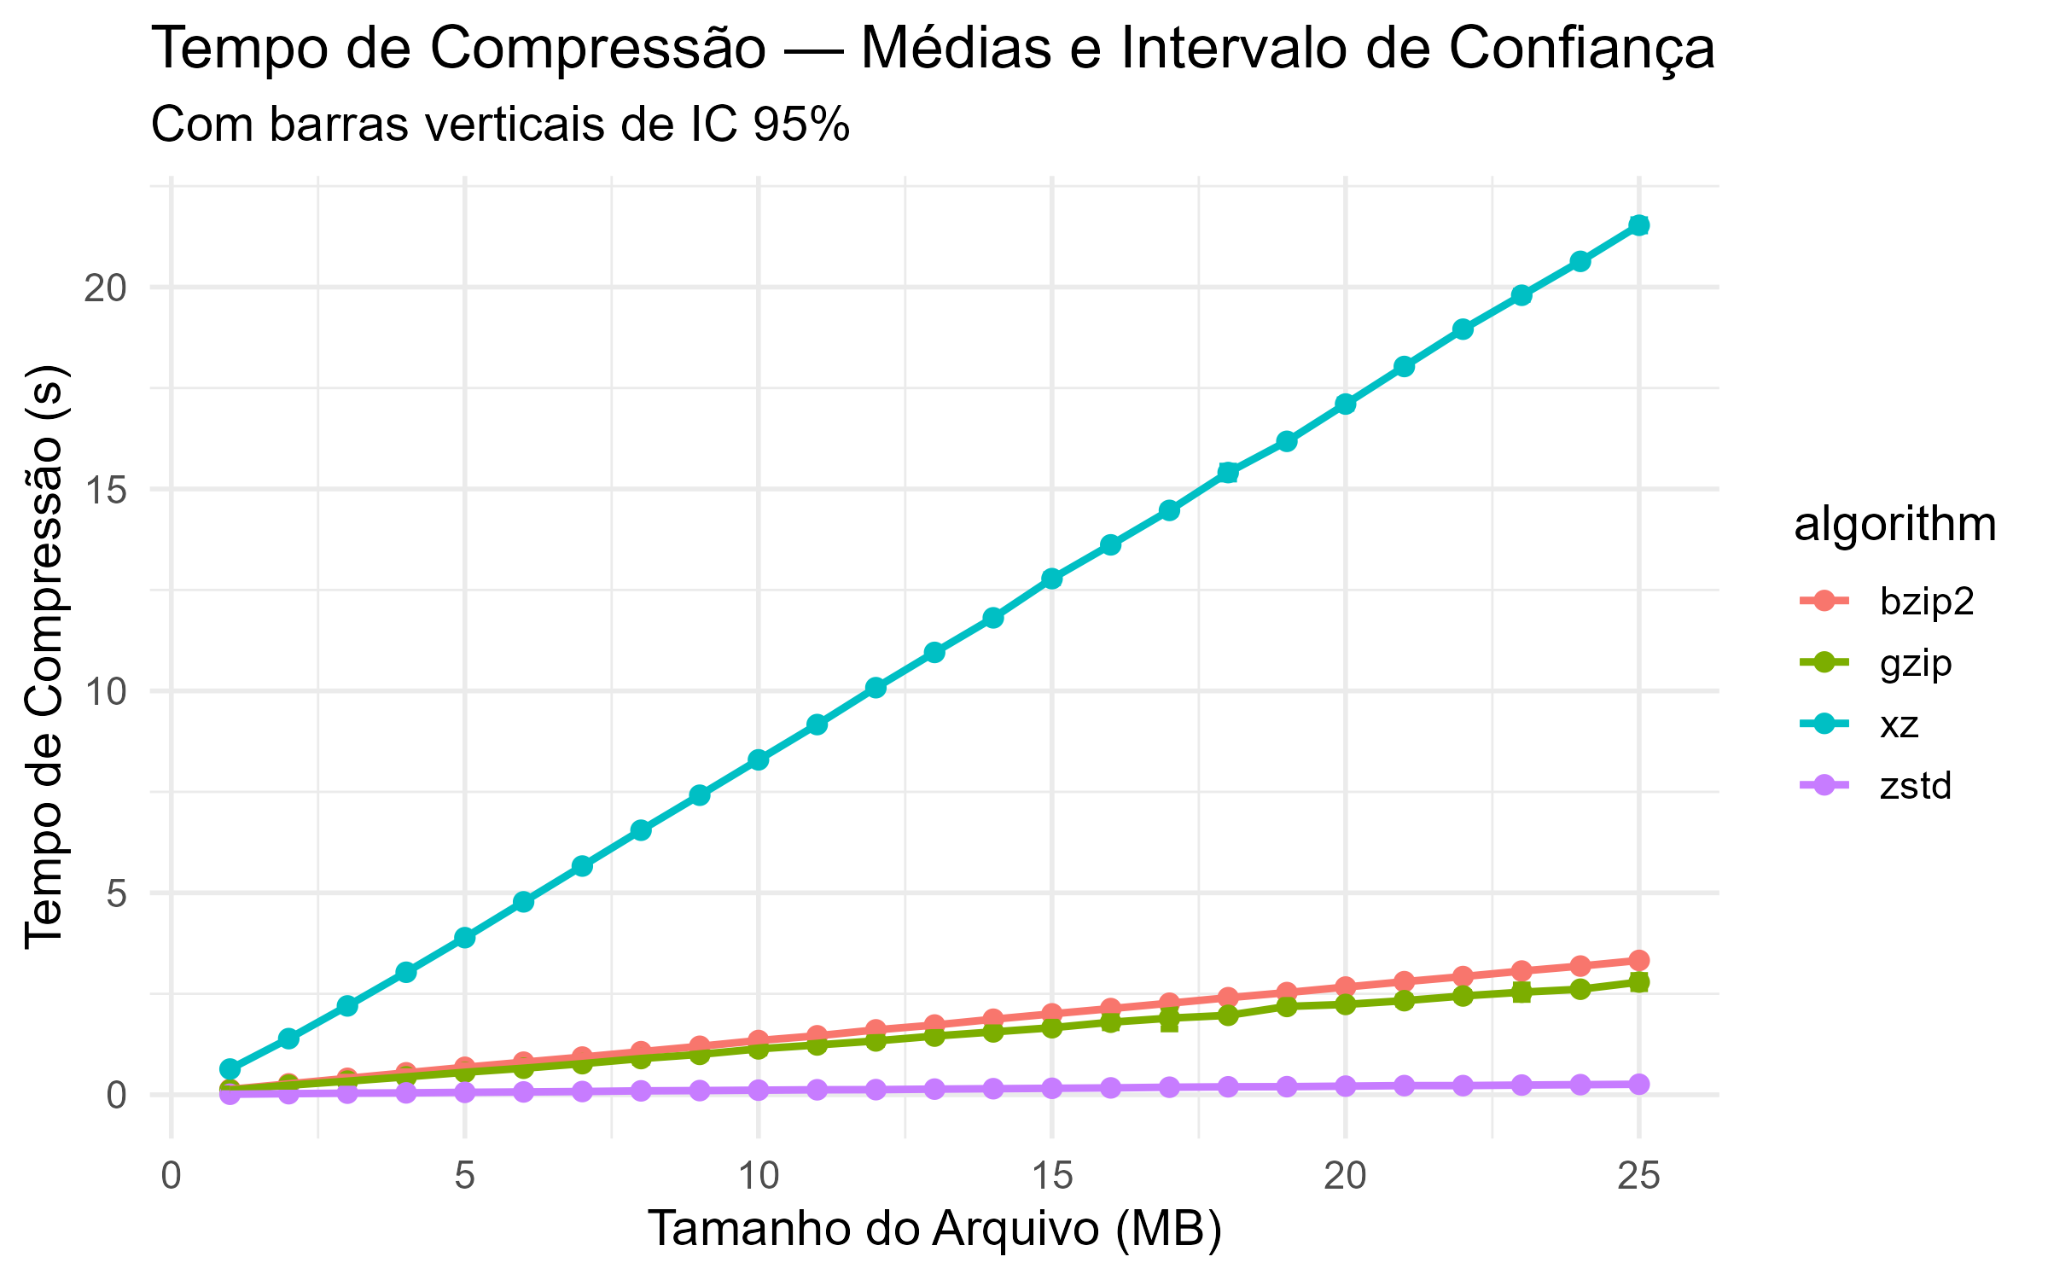
\includegraphics[width=\linewidth]{figures/image10}
  \caption{Tempo de compressão com médias e intervalo de confiança de 95\% (barras verticais).}
  \Description{Gráfico com médias e barras de IC 95\% para tempo de compressão.}
  \label{fig:ic_comp2}
\end{figure}

\begin{figure}[h]
  \centering
  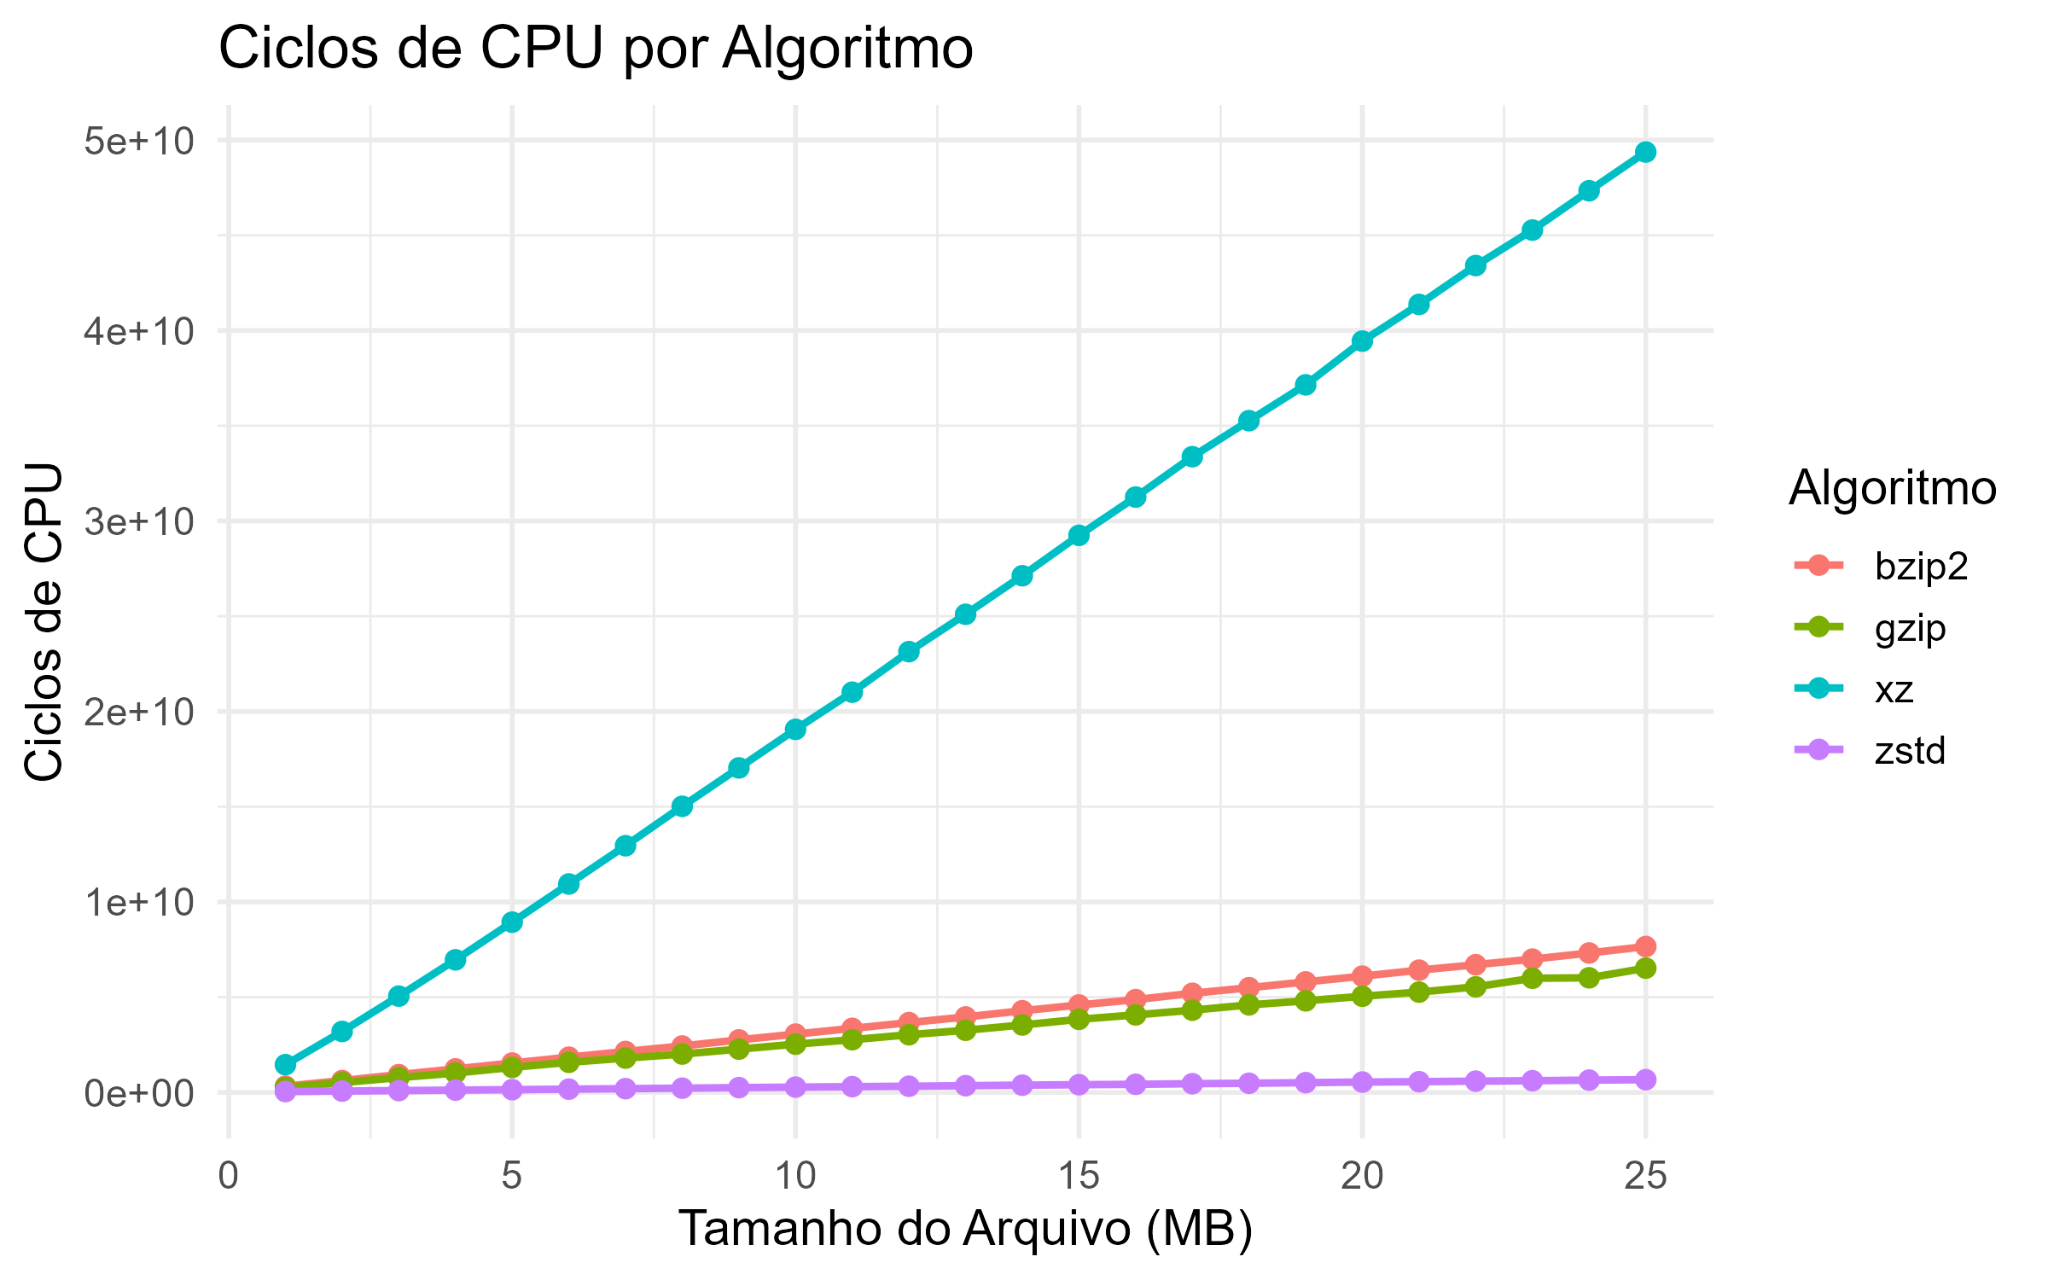
\includegraphics[width=\linewidth]{figures/image12}
  \caption{Intervalo de confiança (95\%) para tempo de descompressão.}
  \Description{Gráfico com barras de erro para tempo de descompressão.}
  \label{fig:ic_decomp}
\end{figure}

%%
%% 5. Discussão
%%
\section{Discussão}

\subsection{Resumo Comparativo dos Algoritmos}

A Tabela~\ref{tab:classificacao} apresenta uma classificação qualitativa dos algoritmos nas principais métricas avaliadas.

\begin{table}[h]
  \centering
  \caption{Classificação dos algoritmos por métrica de desempenho.}
  \label{tab:classificacao}
  \begin{tabular}{lcccc}
    \toprule
    \textbf{Métrica} & \textbf{gzip} & \textbf{bzip2} & \textbf{xz} & \textbf{zstd} \\
    \midrule
    Velocidade de Compressão & Bom & Regular & Ruim & Excelente \\
    Velocidade de Descompressão & Bom & Ruim & Bom & Excelente \\
    Taxa de Compressão & Regular & Bom & Excelente & Bom \\
    Uso de CPU & Baixo & Alto & Muito Alto & Muito Baixo \\
    \midrule
    \textbf{Avaliação Geral} & Bom & Regular & Especializado & Excelente \\
    \bottomrule
  \end{tabular}
\end{table}

A Tabela~\ref{tab:valores} apresenta os valores médios e desvio padrão obtidos considerando todos os tamanhos de arquivo (1MB a 25MB), totalizando 75 amostras por algoritmo.

\begin{table}[h]
  \centering
  \caption{Valores médios e desvio padrão para arquivos de 1--25MB (75 amostras por algoritmo).}
  \label{tab:valores}
  \begin{tabular}{lccc}
    \toprule
    \textbf{Algoritmo} & \textbf{Compressão (ms)} & \textbf{Descompressão (ms)} & \textbf{Taxa (\%)} \\
    \midrule
    gzip & 1448 $\pm$ 805 & 130 $\pm$ 73 & 37,35 $\pm$ 0,04 \\
    bzip2 & 1734 $\pm$ 964 & 869 $\pm$ 487 & 21,68 $\pm$ 0,28 \\
    xz & 10975 $\pm$ 6376 & 117 $\pm$ 57 & 11,88 $\pm$ 2,63 \\
    zstd & 141 $\pm$ 74 & 39 $\pm$ 19 & 24,05 $\pm$ 1,15 \\
    \bottomrule
  \end{tabular}
\end{table}

\subsection{Análise dos Trade-offs}

Os resultados obtidos confirmam os trade-offs conhecidos entre os algoritmos de compressão:

\textbf{gzip} oferece um equilíbrio razoável entre velocidade e simplicidade, sendo ideal para cenários onde compatibilidade é essencial. Entretanto, sua taxa de compressão é a mais baixa entre os algoritmos testados.

\textbf{bzip2} apresenta melhor taxa de compressão que o gzip, mas com penalidade significativa no tempo de descompressão (até 7x mais lento que gzip). É adequado para arquivamento de longo prazo onde a descompressão é infrequente.

\textbf{xz} oferece as melhores taxas de compressão (redução de até 90\%), mas com os maiores tempos de processamento. Recomendado para distribuição de software e arquivos que serão descomprimidos muitas vezes após uma única compressão.

\textbf{zstd} demonstra ser a alternativa mais moderna e versátil, oferecendo velocidades até 80x superiores ao xz com taxas de compressão competitivas. É particularmente adequado para aplicações em tempo real, backups incrementais e streaming de dados.

%%
%% 6. Conclusão
%%
\section{Conclusão}

Este trabalho apresentou uma análise comparativa detalhada de quatro algoritmos de compressão de arquivos: gzip, bzip2, xz e zstd. Através de experimentos controlados em ambiente Docker, foram coletadas métricas de tempo de compressão, descompressão e taxa de compressão para arquivos de texto de 1MB a 25MB.

Os resultados demonstram que não existe um algoritmo universalmente superior, mas sim diferentes trade-offs que devem ser considerados conforme o caso de uso específico. Com base nos experimentos realizados, recomendamos:

\begin{itemize}
  \item \textbf{Para velocidade máxima:} zstd --- até 80x mais rápido que xz na compressão e 24x mais rápido que bzip2 na descompressão.
  \item \textbf{Para melhor taxa de compressão:} xz --- atinge taxas de até 90\%, reduzindo arquivos de 25MB para apenas 2,5MB.
  \item \textbf{Para uso geral moderno:} zstd --- combina alta velocidade com boa taxa de compressão, sendo a escolha mais equilibrada.
  \item \textbf{Para compatibilidade legada:} gzip --- amplamente suportado em todos os sistemas Unix-like.
  \item \textbf{Evitar para descompressão frequente:} bzip2 --- seu tempo de descompressão é significativamente maior que os demais.
\end{itemize}

O algoritmo zstd destaca-se como a melhor escolha para a maioria dos cenários modernos, oferecendo o melhor equilíbrio entre velocidade e eficiência de compressão. O xz permanece relevante para casos onde o tamanho final é crítico e o tempo de compressão não é uma restrição.

Como trabalhos futuros, sugerimos:
\begin{itemize}
  \item Análise com diferentes tipos de arquivos (binários, imagens, dados científicos)
  \item Avaliação de diferentes níveis de compressão de cada algoritmo
  \item Medição do consumo de memória durante a compressão
  \item Análise de compressão paralela (multi-threaded)
\end{itemize}

%%
%% Referências
%%
\bibliographystyle{ACM-Reference-Format}
\bibliography{references}

\end{document}
